\documentclass[12pt]{article}
\usepackage[english]{babel}
\usepackage[utf8]{inputenc}
\usepackage{amsmath, amssymb, amsthm}
\usepackage{graphicx}
\usepackage{hyperref}
\usepackage[margin=.75in]{geometry}
\usepackage{xcolor}
\usepackage{tikz}

\setlength{\topmargin}{0pt}
\setlength{\headsep}{0pt}
\textheight = 600pt

\title{Graph Theory \\ Homework 4}
\author{Ben Kallus and Maddy LaPoint}
\date{Due Monday, February 15}

\begin{document}
\maketitle

\noindent{\bf FIRST}

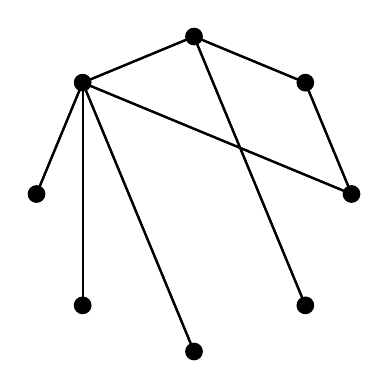
\begin{tikzpicture}
\draw[fill=black] (1.414, 1.414) circle (3pt);
\draw[fill=black] (2.0, 0.0) circle (3pt);
\draw[fill=black] (0.0, 2.0) circle (3pt);
\draw[fill=black] (-1.414, 1.414) circle (3pt);
\draw[fill=black] (-2.0, 0.0) circle (3pt);
\draw[fill=black] (-1.414, -1.414) circle (3pt);
\draw[fill=black] (-0.0, -2.0) circle (3pt);
\draw[fill=black] (1.414, -1.414) circle (3pt);

\draw[thick] (1.414, 1.414) -- (0.0, 2.0);
\draw[thick] (1.414, 1.414) -- (2.0, 0.0);
\draw[thick] (2.0, 0.0) -- (-1.414, 1.414);
\draw[thick] (2.0, 0.0) -- (1.414, 1.414);
\draw[thick] (0.0, 2.0) -- (-1.414, 1.414);
\draw[thick] (0.0, 2.0) -- (1.414, -1.414);
\draw[thick] (0.0, 2.0) -- (1.414, 1.414);
\draw[thick] (-1.414, 1.414) -- (-2.0, 0.0);
\draw[thick] (-1.414, 1.414) -- (-0.0, -2.0);
\draw[thick] (-1.414, 1.414) -- (0.0, 2.0);
\draw[thick] (-1.414, 1.414) -- (2.0, 0.0);
\draw[thick] (-1.414, 1.414) -- (-1.414, -1.414);
\draw[thick] (-2.0, 0.0) -- (-1.414, 1.414);
\draw[thick] (-1.414, -1.414) -- (-1.414, 1.414);
\draw[thick] (-0.0, -2.0) -- (-1.414, 1.414);
\draw[thick] (1.414, -1.414) -- (0.0, 2.0);
\end{tikzpicture}
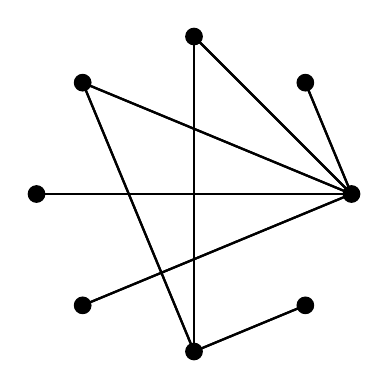
\begin{tikzpicture}
\draw[fill=black] (2.0, 0.0) circle (3pt);
\draw[fill=black] (1.414, 1.414) circle (3pt);
\draw[fill=black] (0.0, 2.0) circle (3pt);
\draw[fill=black] (-1.414, 1.414) circle (3pt);
\draw[fill=black] (-2.0, 0.0) circle (3pt);
\draw[fill=black] (-1.414, -1.414) circle (3pt);
\draw[fill=black] (-0.0, -2.0) circle (3pt);
\draw[fill=black] (1.414, -1.414) circle (3pt);

\draw[thick] (2.0, 0.0) -- (-1.414, 1.414);
\draw[thick] (2.0, 0.0) -- (-1.414, -1.414);
\draw[thick] (2.0, 0.0) -- (1.414, 1.414);
\draw[thick] (2.0, 0.0) -- (0.0, 2.0);
\draw[thick] (2.0, 0.0) -- (-2.0, 0.0);
\draw[thick] (1.414, 1.414) -- (2.0, 0.0);
\draw[thick] (0.0, 2.0) -- (-0.0, -2.0);
\draw[thick] (0.0, 2.0) -- (2.0, 0.0);
\draw[thick] (-1.414, 1.414) -- (-0.0, -2.0);
\draw[thick] (-1.414, 1.414) -- (2.0, 0.0);
\draw[thick] (-2.0, 0.0) -- (2.0, 0.0);
\draw[thick] (-1.414, -1.414) -- (2.0, 0.0);
\draw[thick] (-0.0, -2.0) -- (-1.414, 1.414);
\draw[thick] (-0.0, -2.0) -- (0.0, 2.0);
\draw[thick] (-0.0, -2.0) -- (1.414, -1.414);
\draw[thick] (1.414, -1.414) -- (-0.0, -2.0);
\end{tikzpicture}
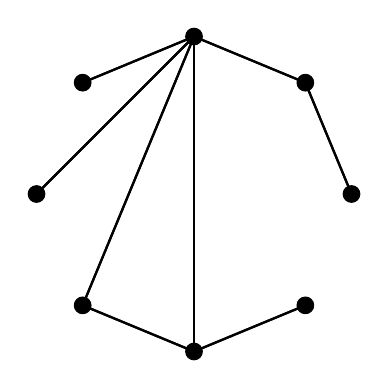
\begin{tikzpicture}
\draw[fill=black] (2.0, 0.0) circle (3pt);
\draw[fill=black] (1.414, 1.414) circle (3pt);
\draw[fill=black] (0.0, 2.0) circle (3pt);
\draw[fill=black] (-1.414, 1.414) circle (3pt);
\draw[fill=black] (-2.0, 0.0) circle (3pt);
\draw[fill=black] (-1.414, -1.414) circle (3pt);
\draw[fill=black] (-0.0, -2.0) circle (3pt);
\draw[fill=black] (1.414, -1.414) circle (3pt);

\draw[thick] (2.0, 0.0) -- (1.414, 1.414);
\draw[thick] (1.414, 1.414) -- (2.0, 0.0);
\draw[thick] (1.414, 1.414) -- (0.0, 2.0);
\draw[thick] (0.0, 2.0) -- (-0.0, -2.0);
\draw[thick] (0.0, 2.0) -- (-1.414, 1.414);
\draw[thick] (0.0, 2.0) -- (-1.414, -1.414);
\draw[thick] (0.0, 2.0) -- (1.414, 1.414);
\draw[thick] (0.0, 2.0) -- (-2.0, 0.0);
\draw[thick] (-1.414, 1.414) -- (0.0, 2.0);
\draw[thick] (-2.0, 0.0) -- (0.0, 2.0);
\draw[thick] (-1.414, -1.414) -- (-0.0, -2.0);
\draw[thick] (-1.414, -1.414) -- (0.0, 2.0);
\draw[thick] (-0.0, -2.0) -- (1.414, -1.414);
\draw[thick] (-0.0, -2.0) -- (-1.414, -1.414);
\draw[thick] (-0.0, -2.0) -- (0.0, 2.0);
\draw[thick] (1.414, -1.414) -- (-0.0, -2.0);
\end{tikzpicture}

\newpage\noindent{\bf 2.31} Proposition: The degree sequence $(d_1, d_2, \hdots, d_n)$ is graphical if and only if the degree sequence $(n-d_n-1, n-d_{n-1}-1, \hdots, n-d_1-1)$ is graphical.
\begin{proof}
    Suppose that the degree sequence $D = (d_1, d_2, \hdots, d_n)$ is graphical.
    Then, there exists a graph $G$ of order $n$ with degree sequence $D$.
    Let $v \in V(G)$.
    Then, $\deg(v) = d_m$, for some $m \in \mathbb N$ satisfying $1 \leq m \leq n$.
    By the definition of $\overline G$, $$\deg_{\overline{G}}(v) + \deg_G(v) = n-1.$$
    Then, $$\deg_{\overline{G}}(v) = n - \deg_G(v) - 1.$$
    Therefore, $$\deg_{\overline{G}}(v) = n - d_m - 1.$$
    Thus, $D' = (n-d_n-1, n-d_{n-1}-1, \hdots, n-d_1-1)$ is the degree sequence for $\overline G$, so $D'$ is graphical.

    Now, suppose that the degree sequence $D' = (n-d_n-1, n-d_{n-1}-1, \hdots, n-d_1-1)$ is graphical.
    Then, by the result of the previous direction of this proof, the degree sequence
    \begin{align*}
        D'' &= (n-(n-d_1-1)-1, n-(n-d_2-1)-1, \hdots, n-(n-d_n-1)-1) \\
            &= (n-n+d_1+1-1, n-n+d_2+1-1, \hdots, n-n+d_n+1-1) \\
            &= (d_1, d_2, \hdots, d_n)
    \end{align*} is graphical.
\end{proof}

\newpage\noindent{\bf 2.32}

\medskip{\bf (a)}
\begin{align*}
    s_1  &= (5,3,3,3,3,2,2,2,1) \\
    s_1' &=   (2,2,2,2,2,2,1,1)
\end{align*} Since $s_1'$ is the degree sequence of $C_6 \cup K_2$, $s_1$ is graphical.

Shown left to right are graphs corresponding to $s_1'$ and $s_1$:
\begin{center}
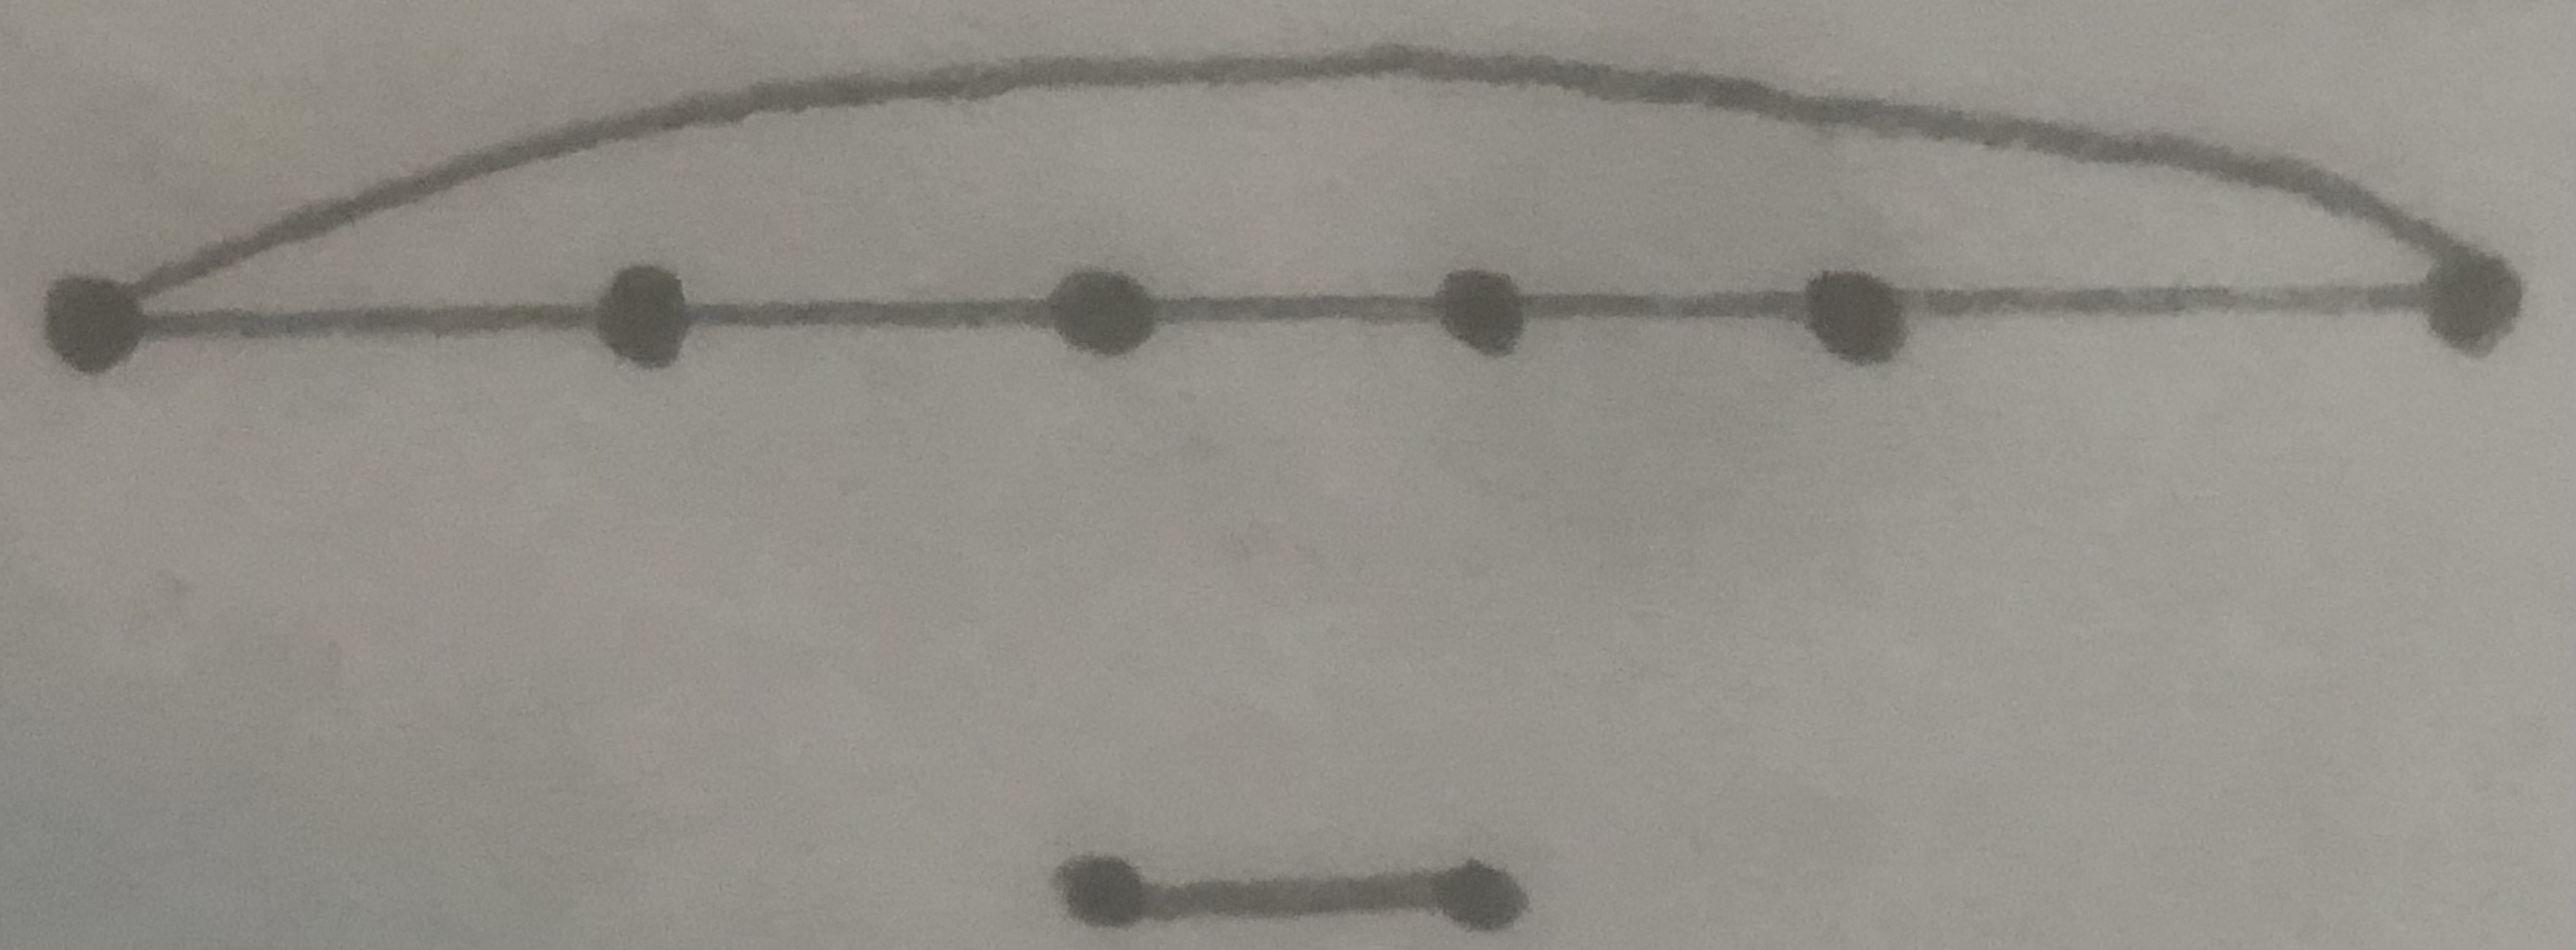
\includegraphics[height=2.7cm]{IMG-0792.JPG}
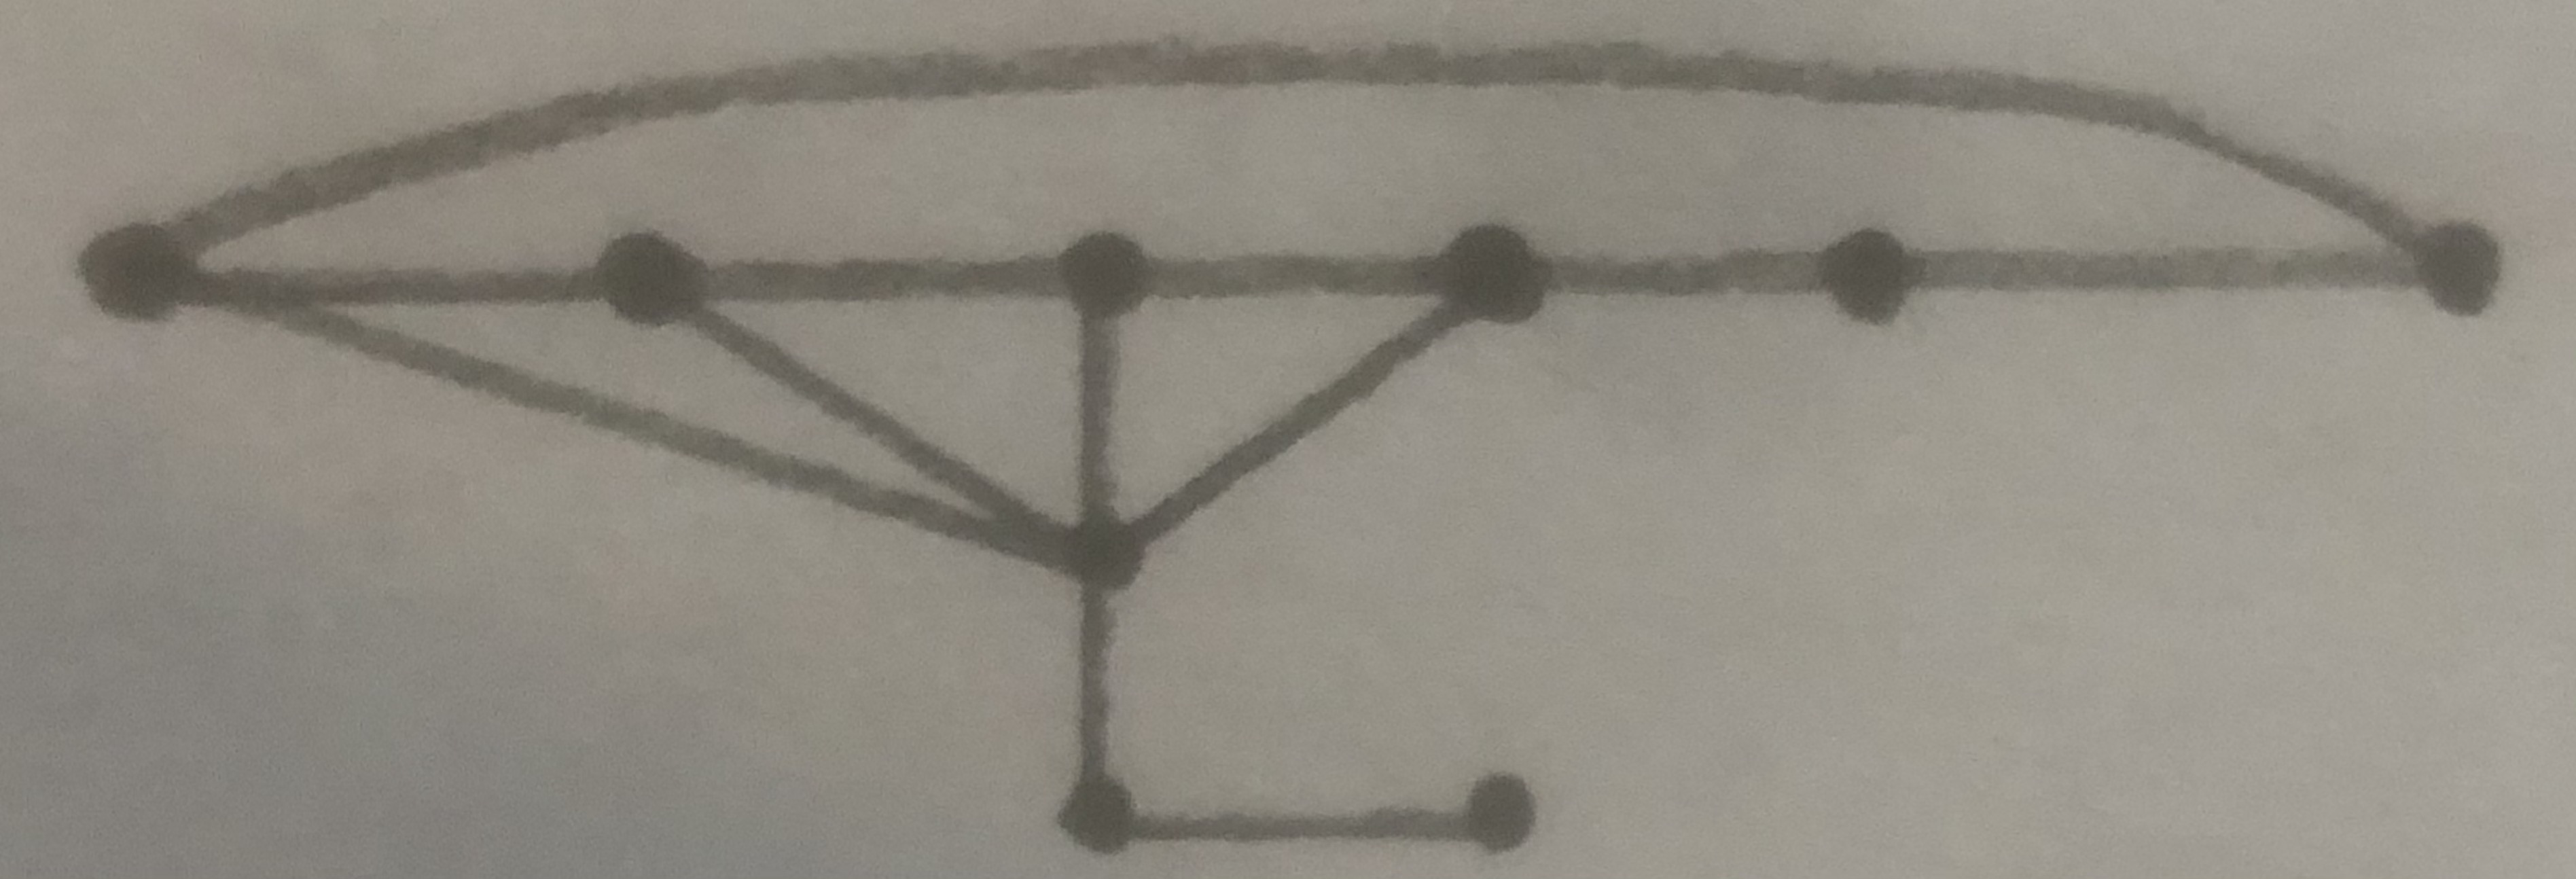
\includegraphics[height=2.5cm]{IMG-0793.JPG}
\end{center}

\medskip{\bf (b)}
\begin{align*}
    s_2  &= (6,3,3,3,3,2,2,2,2,1,1) \\
    s_2' &=   (2,2,2,2,2,2,1,1,1,1)
\end{align*} Since $s_2'$ is the degree sequence of $C_6 \cup 2K_2$, $s_2$ is graphical.

Shown left to right are graphs corresponding to $s_2'$ and $s_2$:
\begin{center}
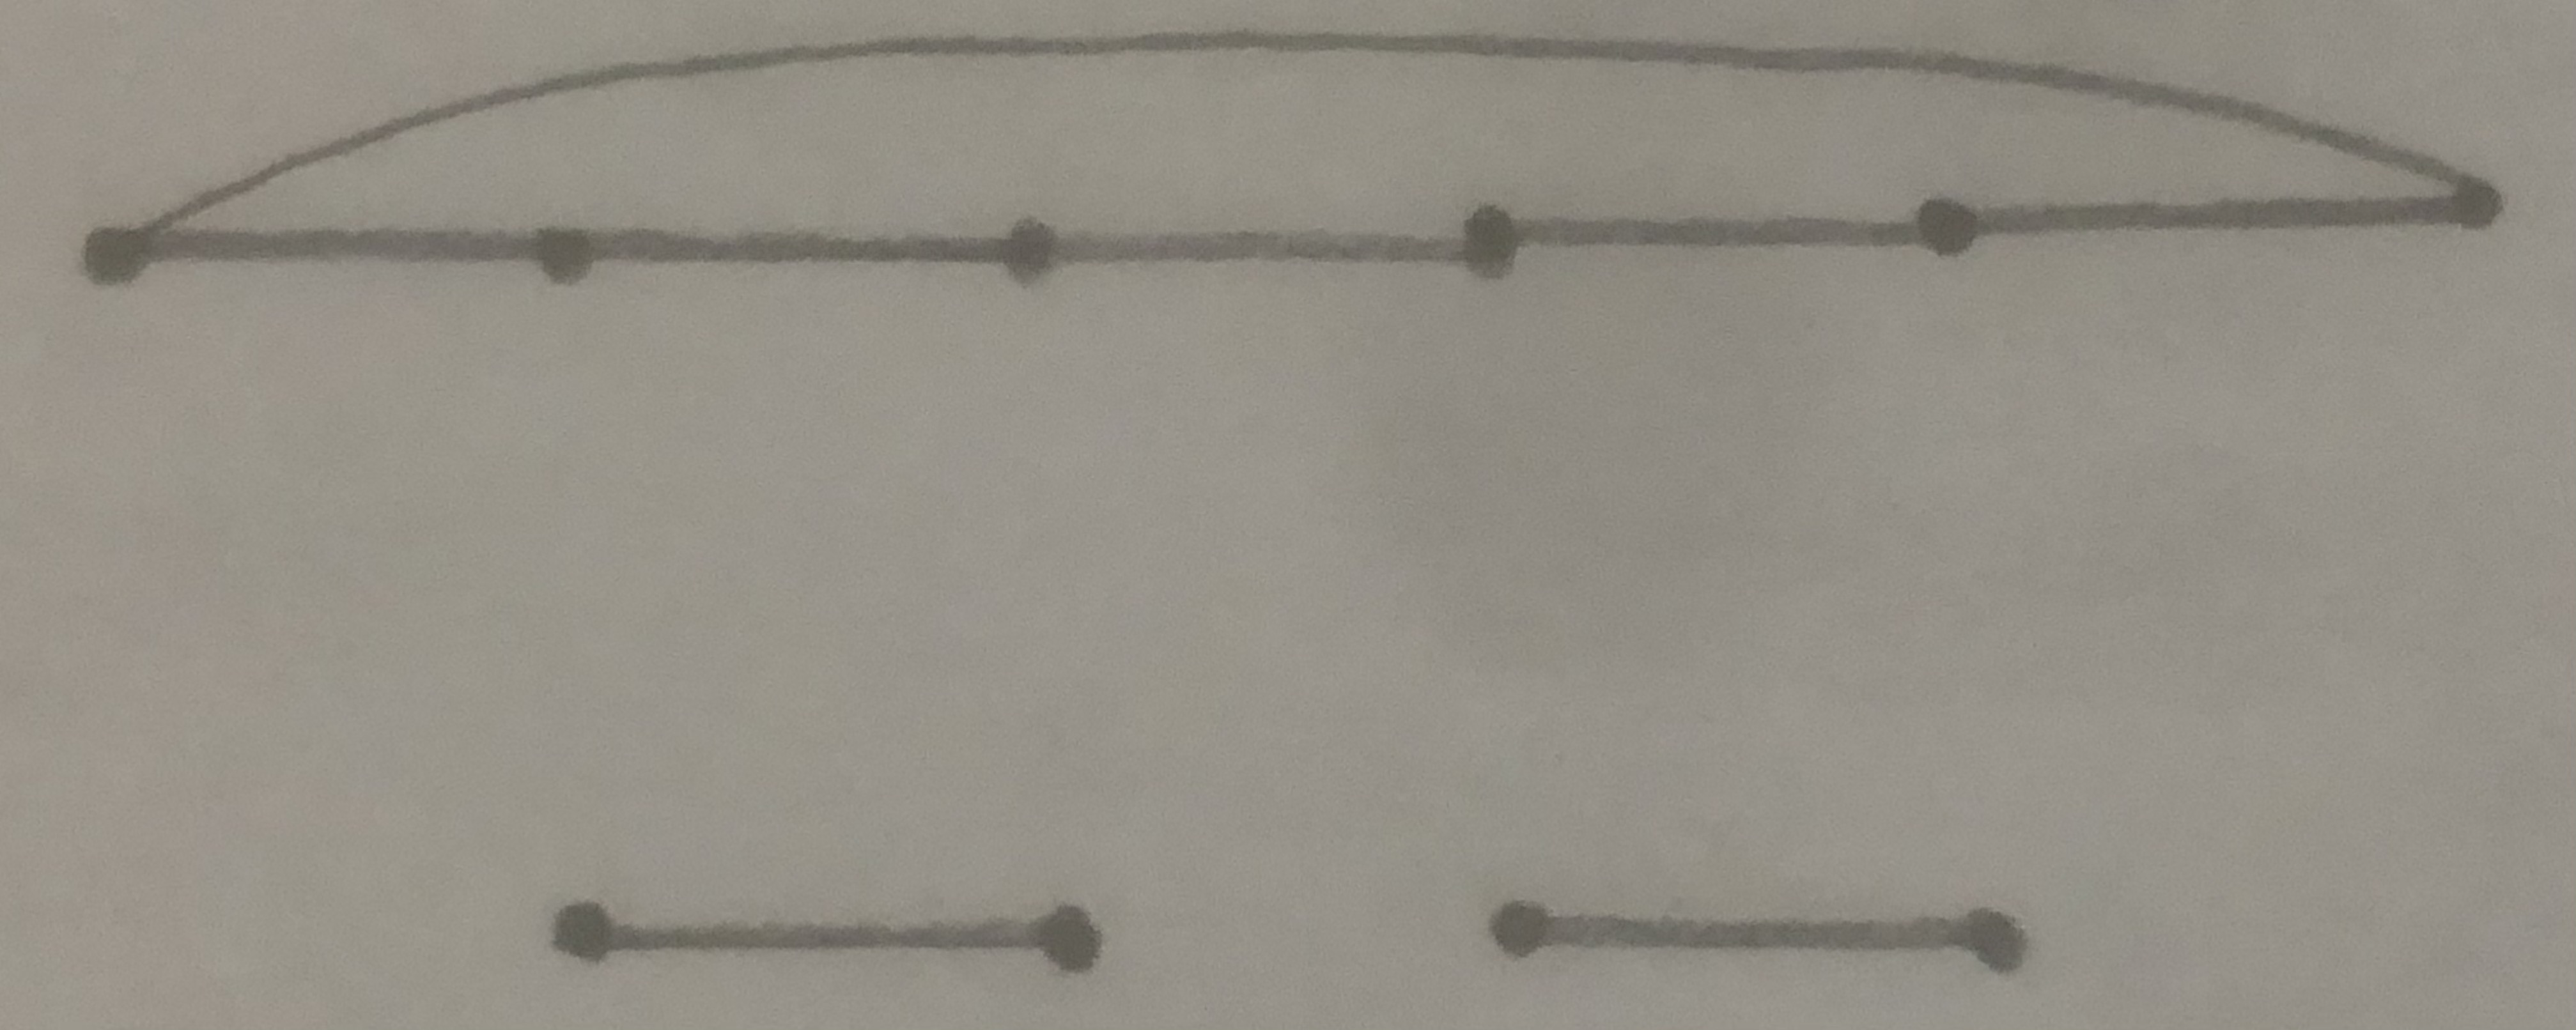
\includegraphics[height=3cm]{IMG-0790.JPG}
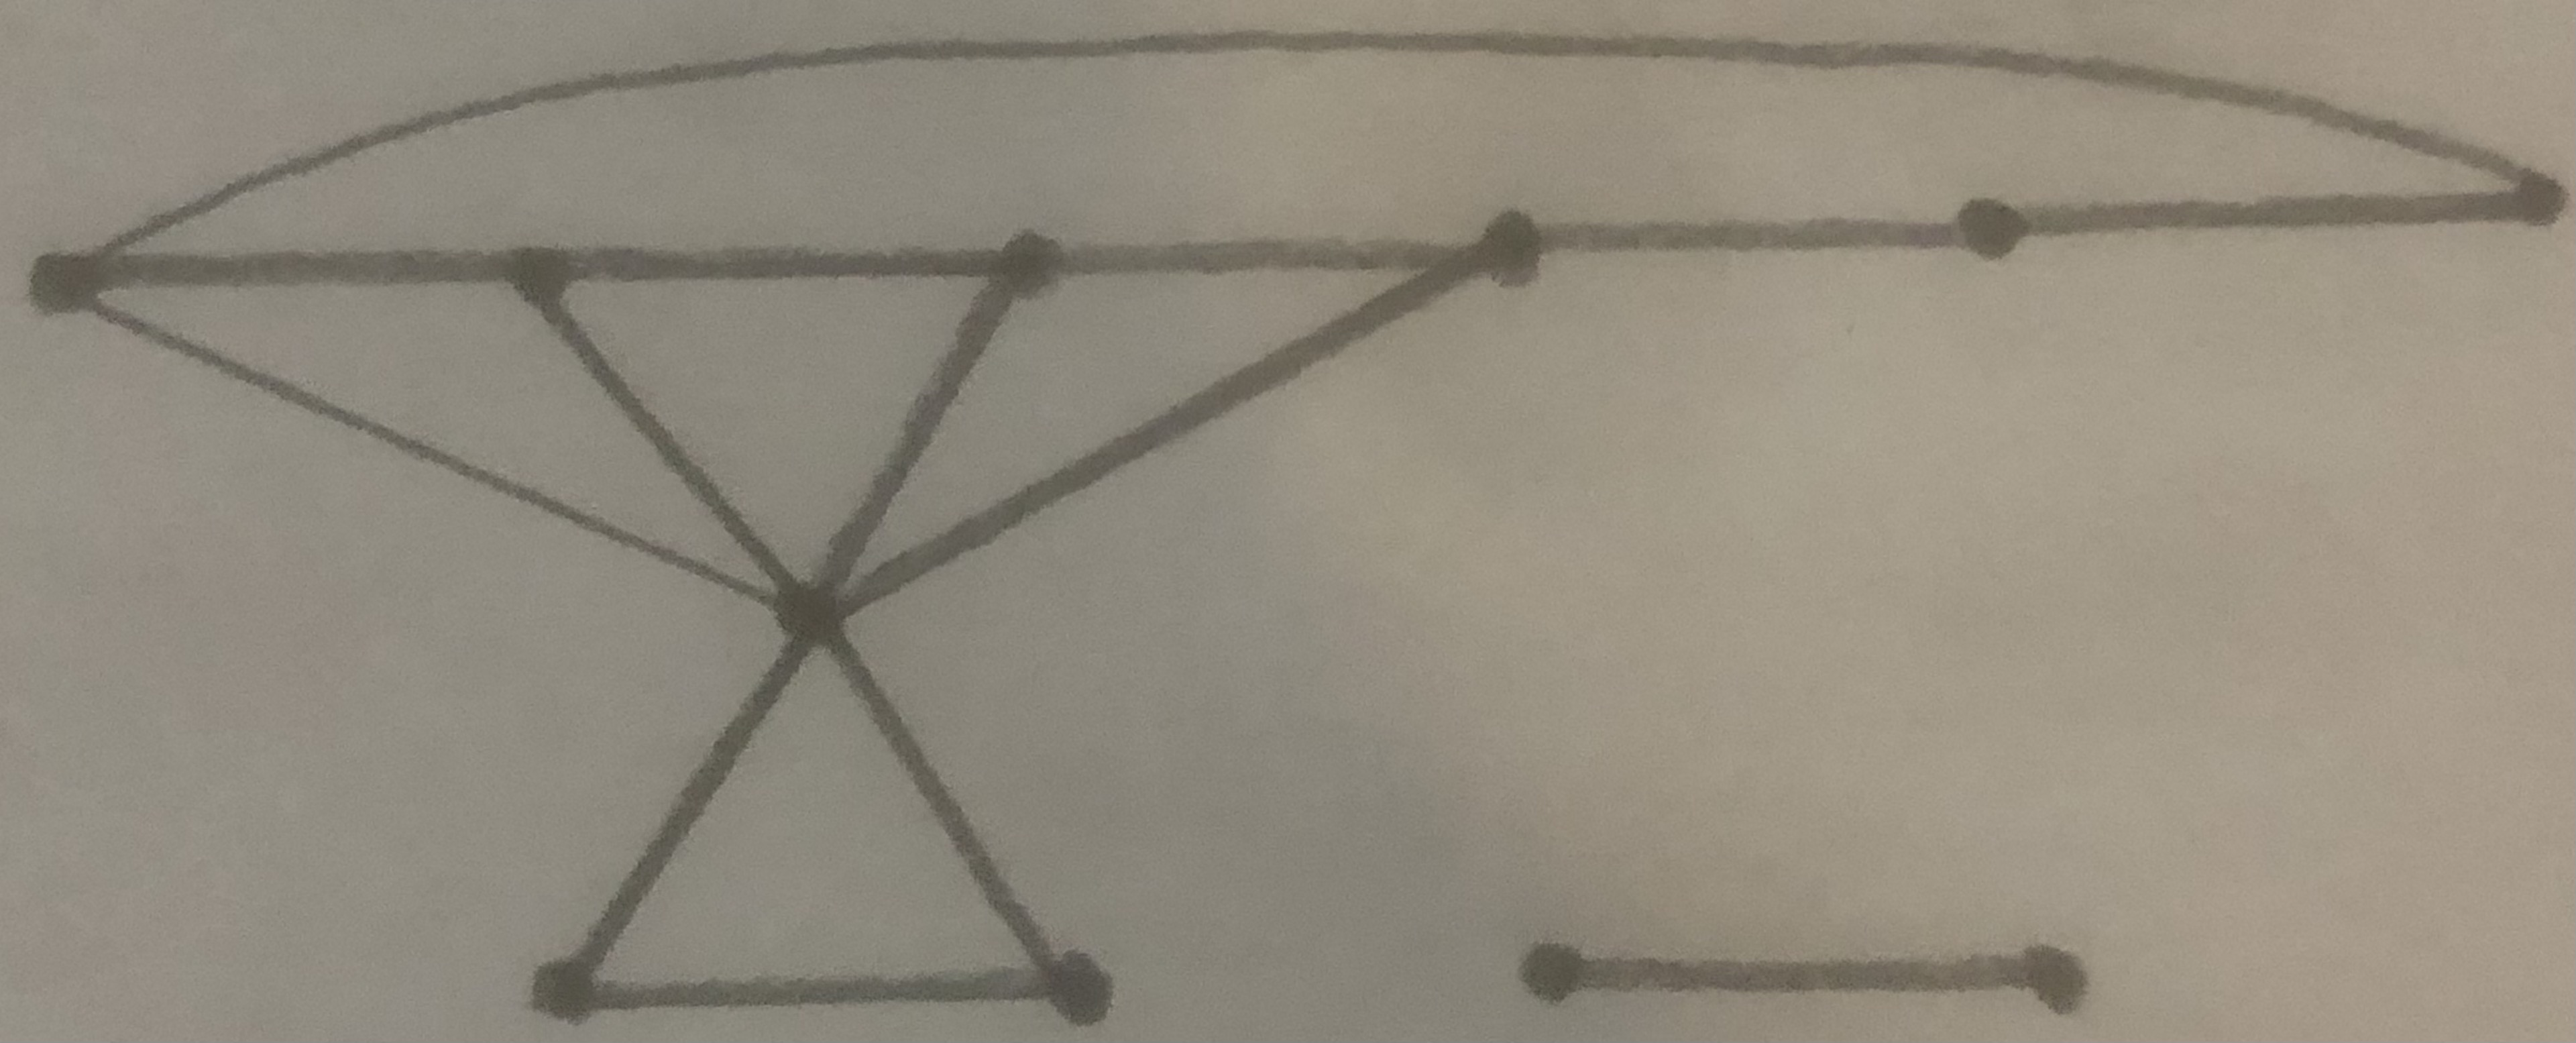
\includegraphics[height=3cm]{IMG-0791.JPG}
\end{center}

\medskip{\bf (c)}
\begin{align*}
    s_3    &= (6,5,5,4,3,2,1) \\
    s_3'   &=   (4,4,3,2,1,0) \\
    s_3''  &=     (3,2,1,0,0)
\end{align*}
$s_3''$ is not graphical because it contains a 3, but does not contain 4 nonzero entries.
Thus, $s_3$ is not graphical.

\newpage{\bf (d)}
\begin{align*}
    s_4   &= (7,5,4,4,4,3,2,1) \\
    s_4'  &=   (4,3,3,3,2,1,0) \\
    s_4'' &=     (2,2,2,1,1,0)
\end{align*} Since $s_4''$ is the degree sequence of $C_3 \cup K_2 \cup N_1$, $s_4$ is graphical.

Shown left to right are graphs corresponding to $s_4''$, $s_4'$, and $s_4$:
\begin{center}
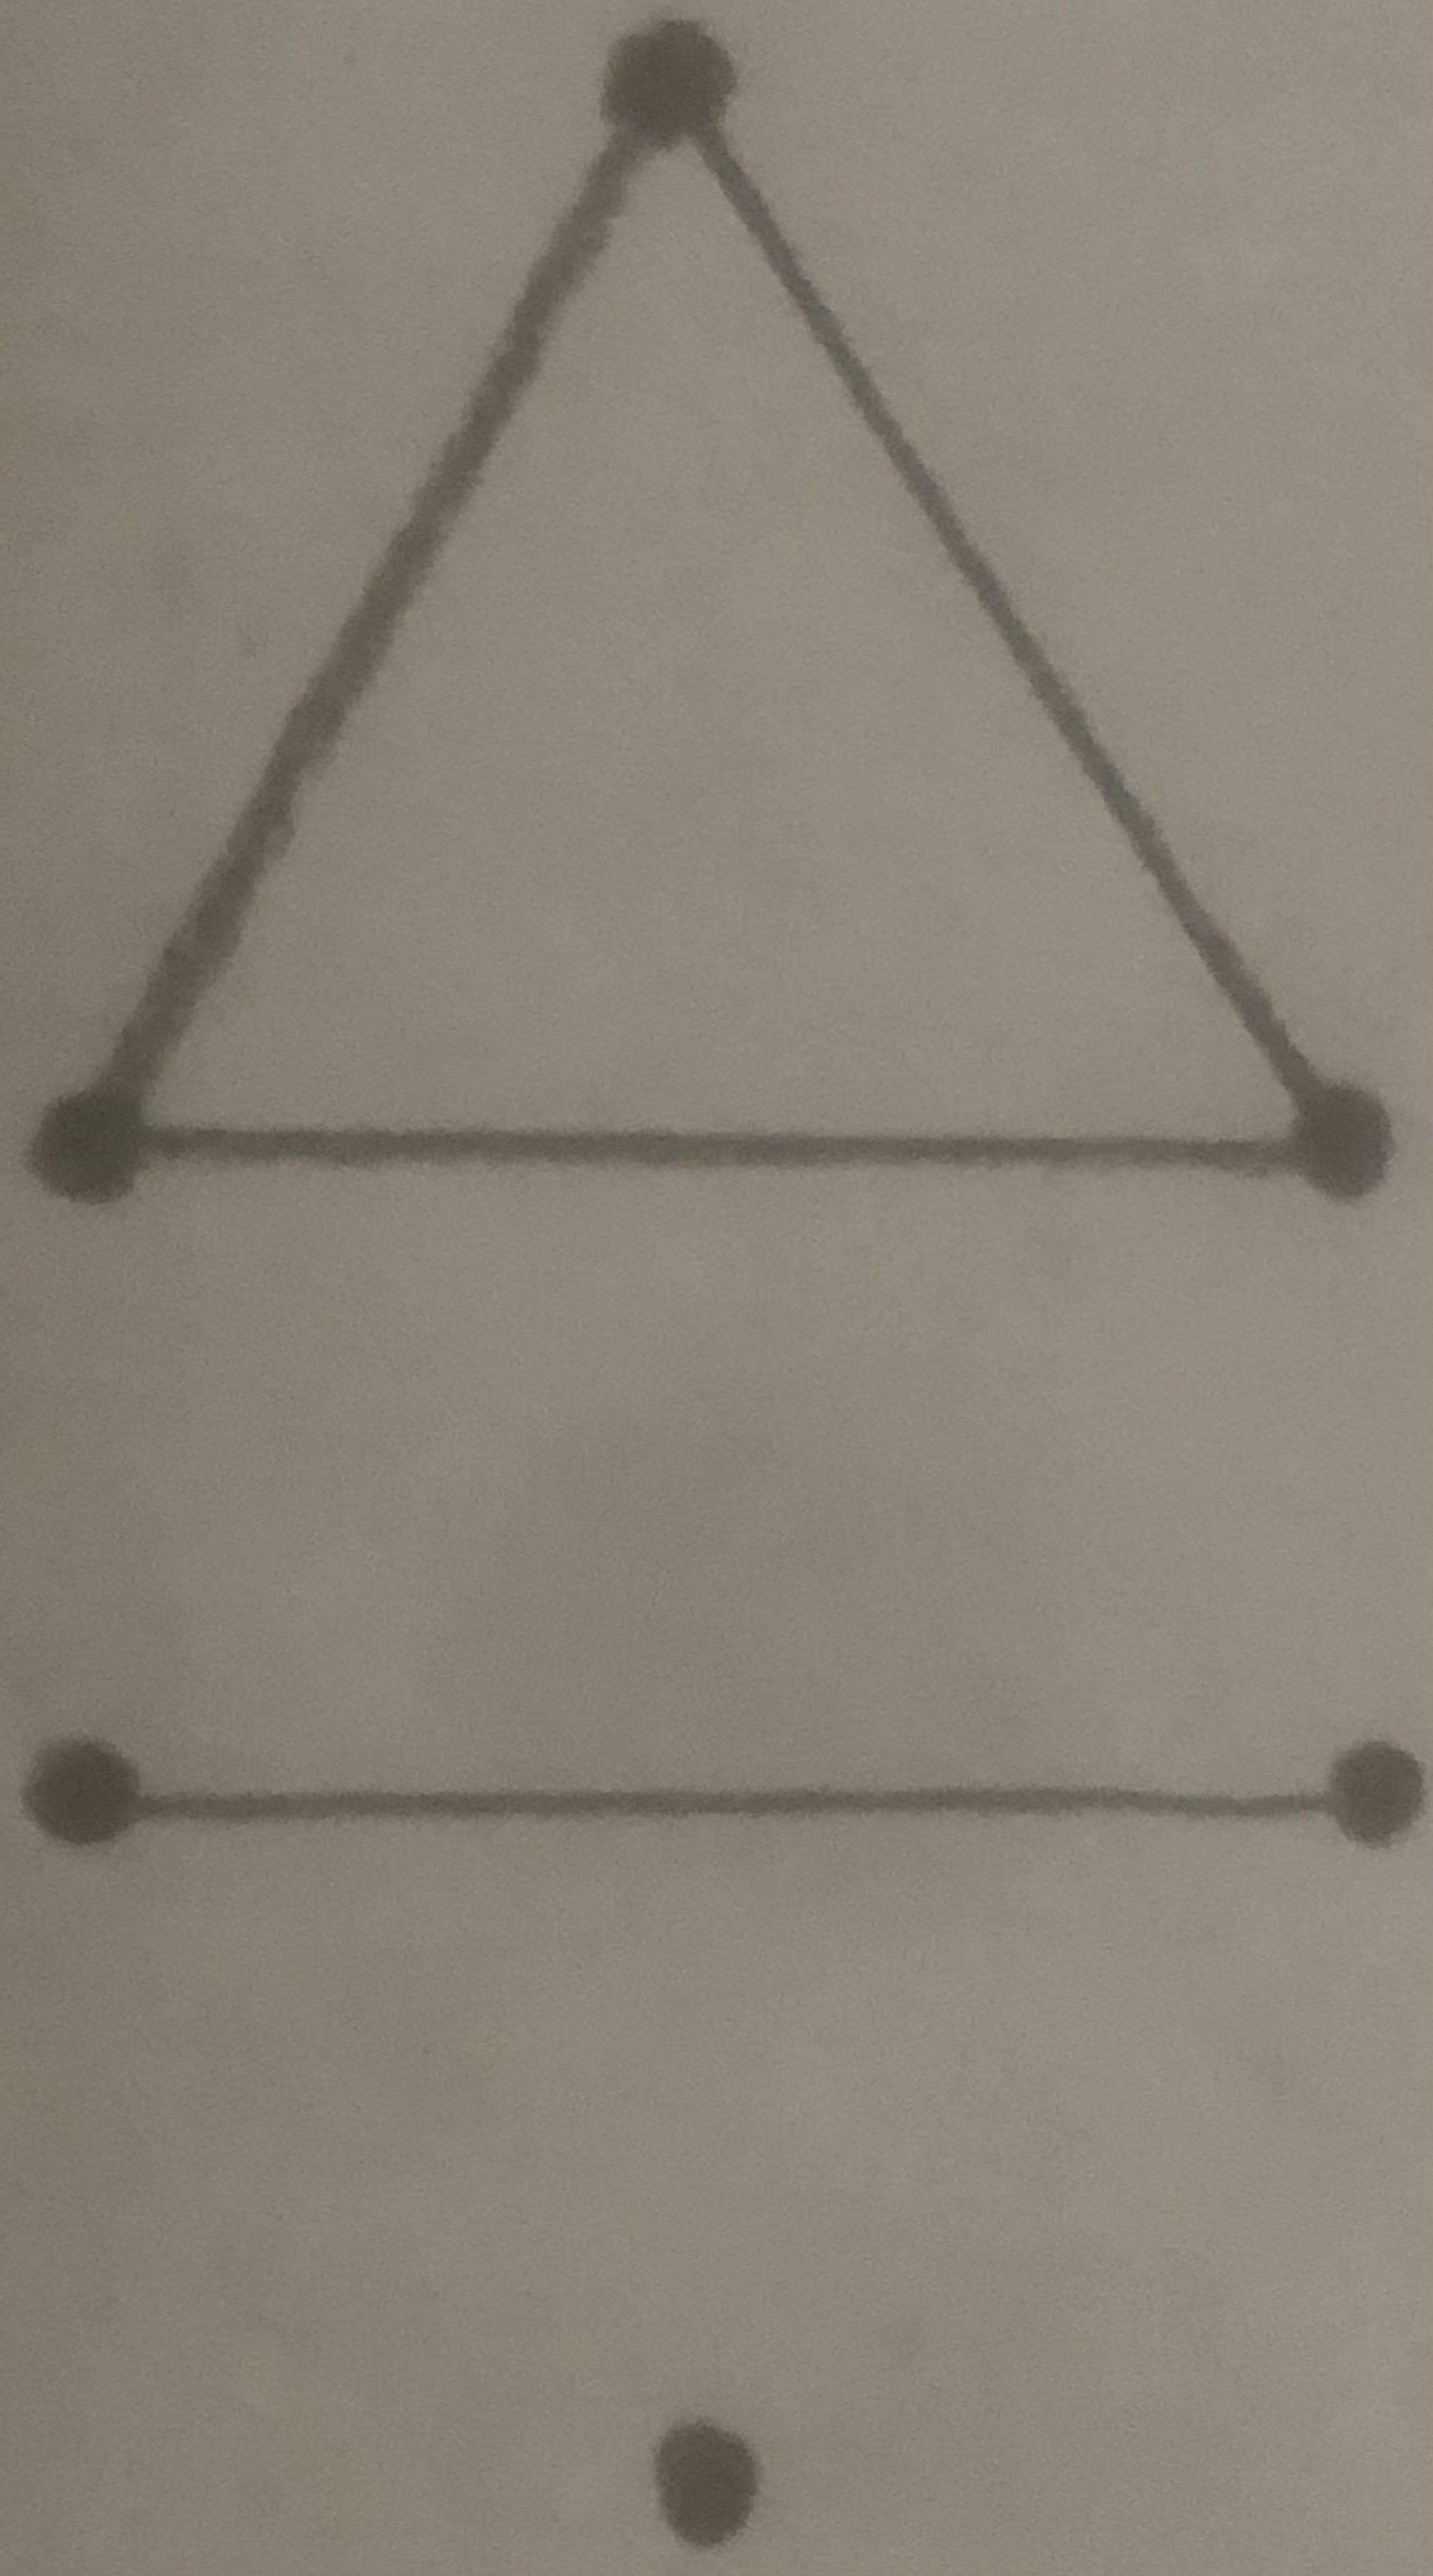
\includegraphics[width=3cm]{IMG-0783.JPG}
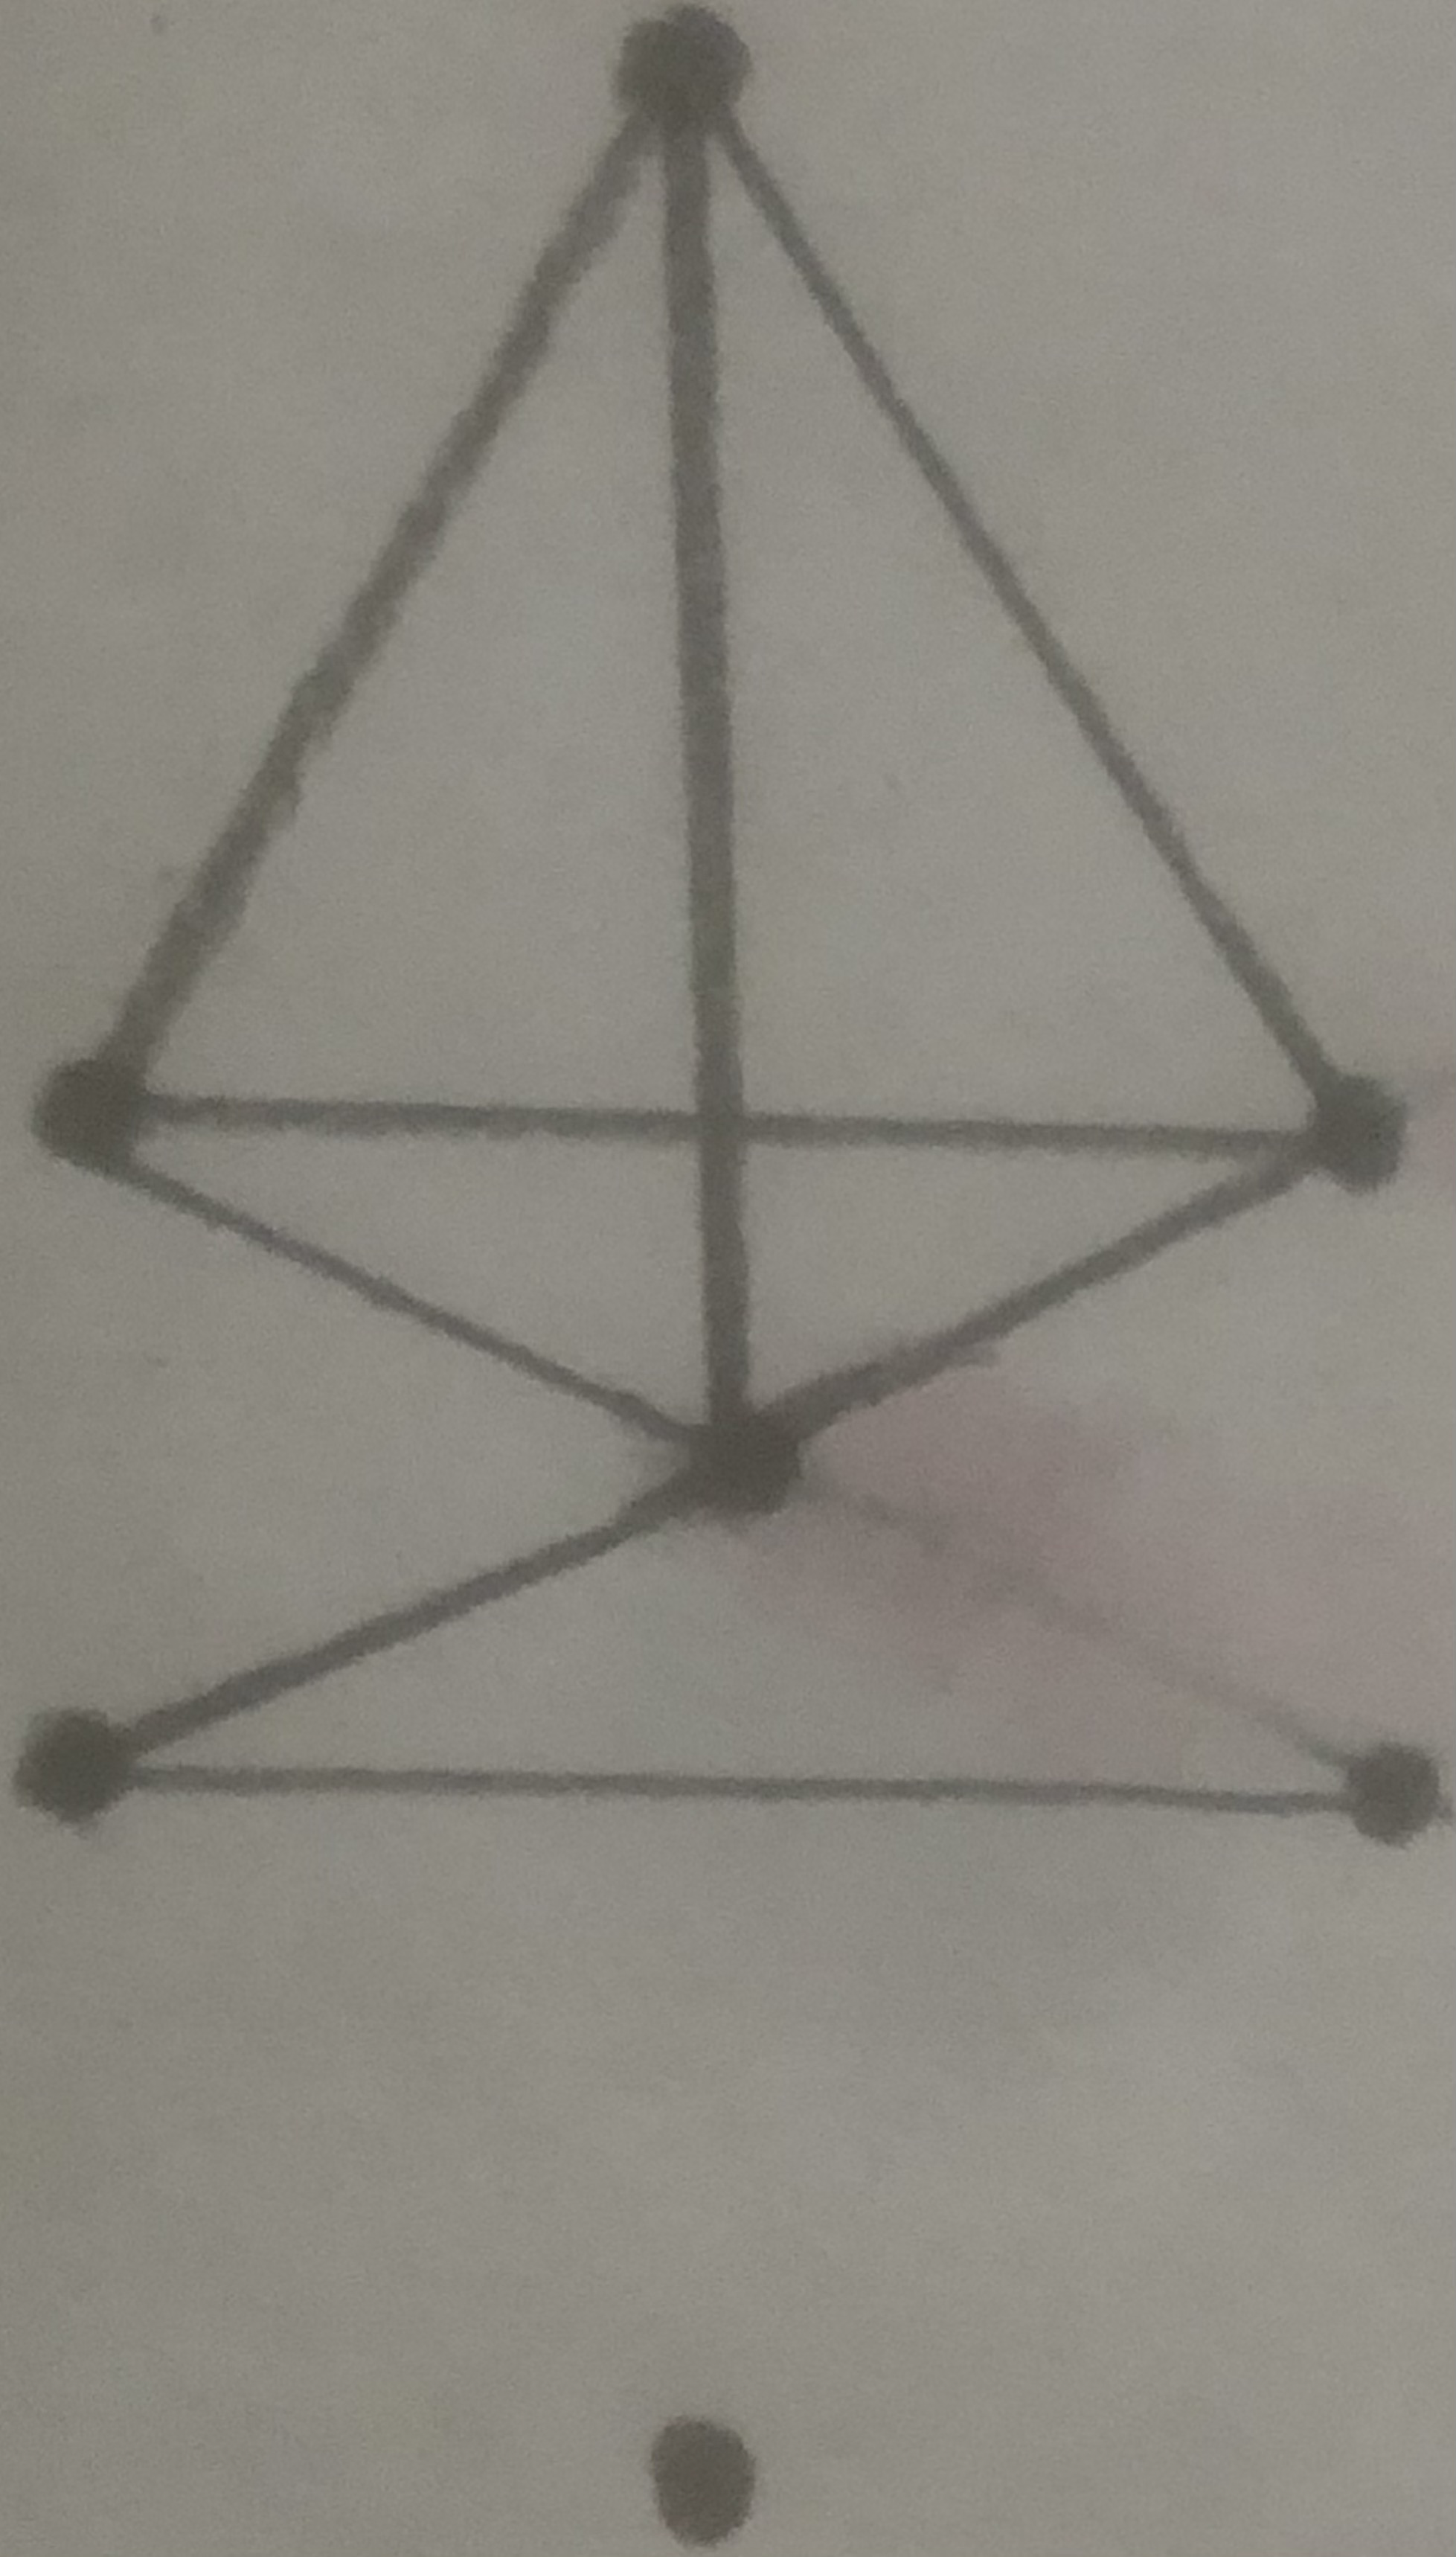
\includegraphics[width=3cm]{IMG-0784.JPG}
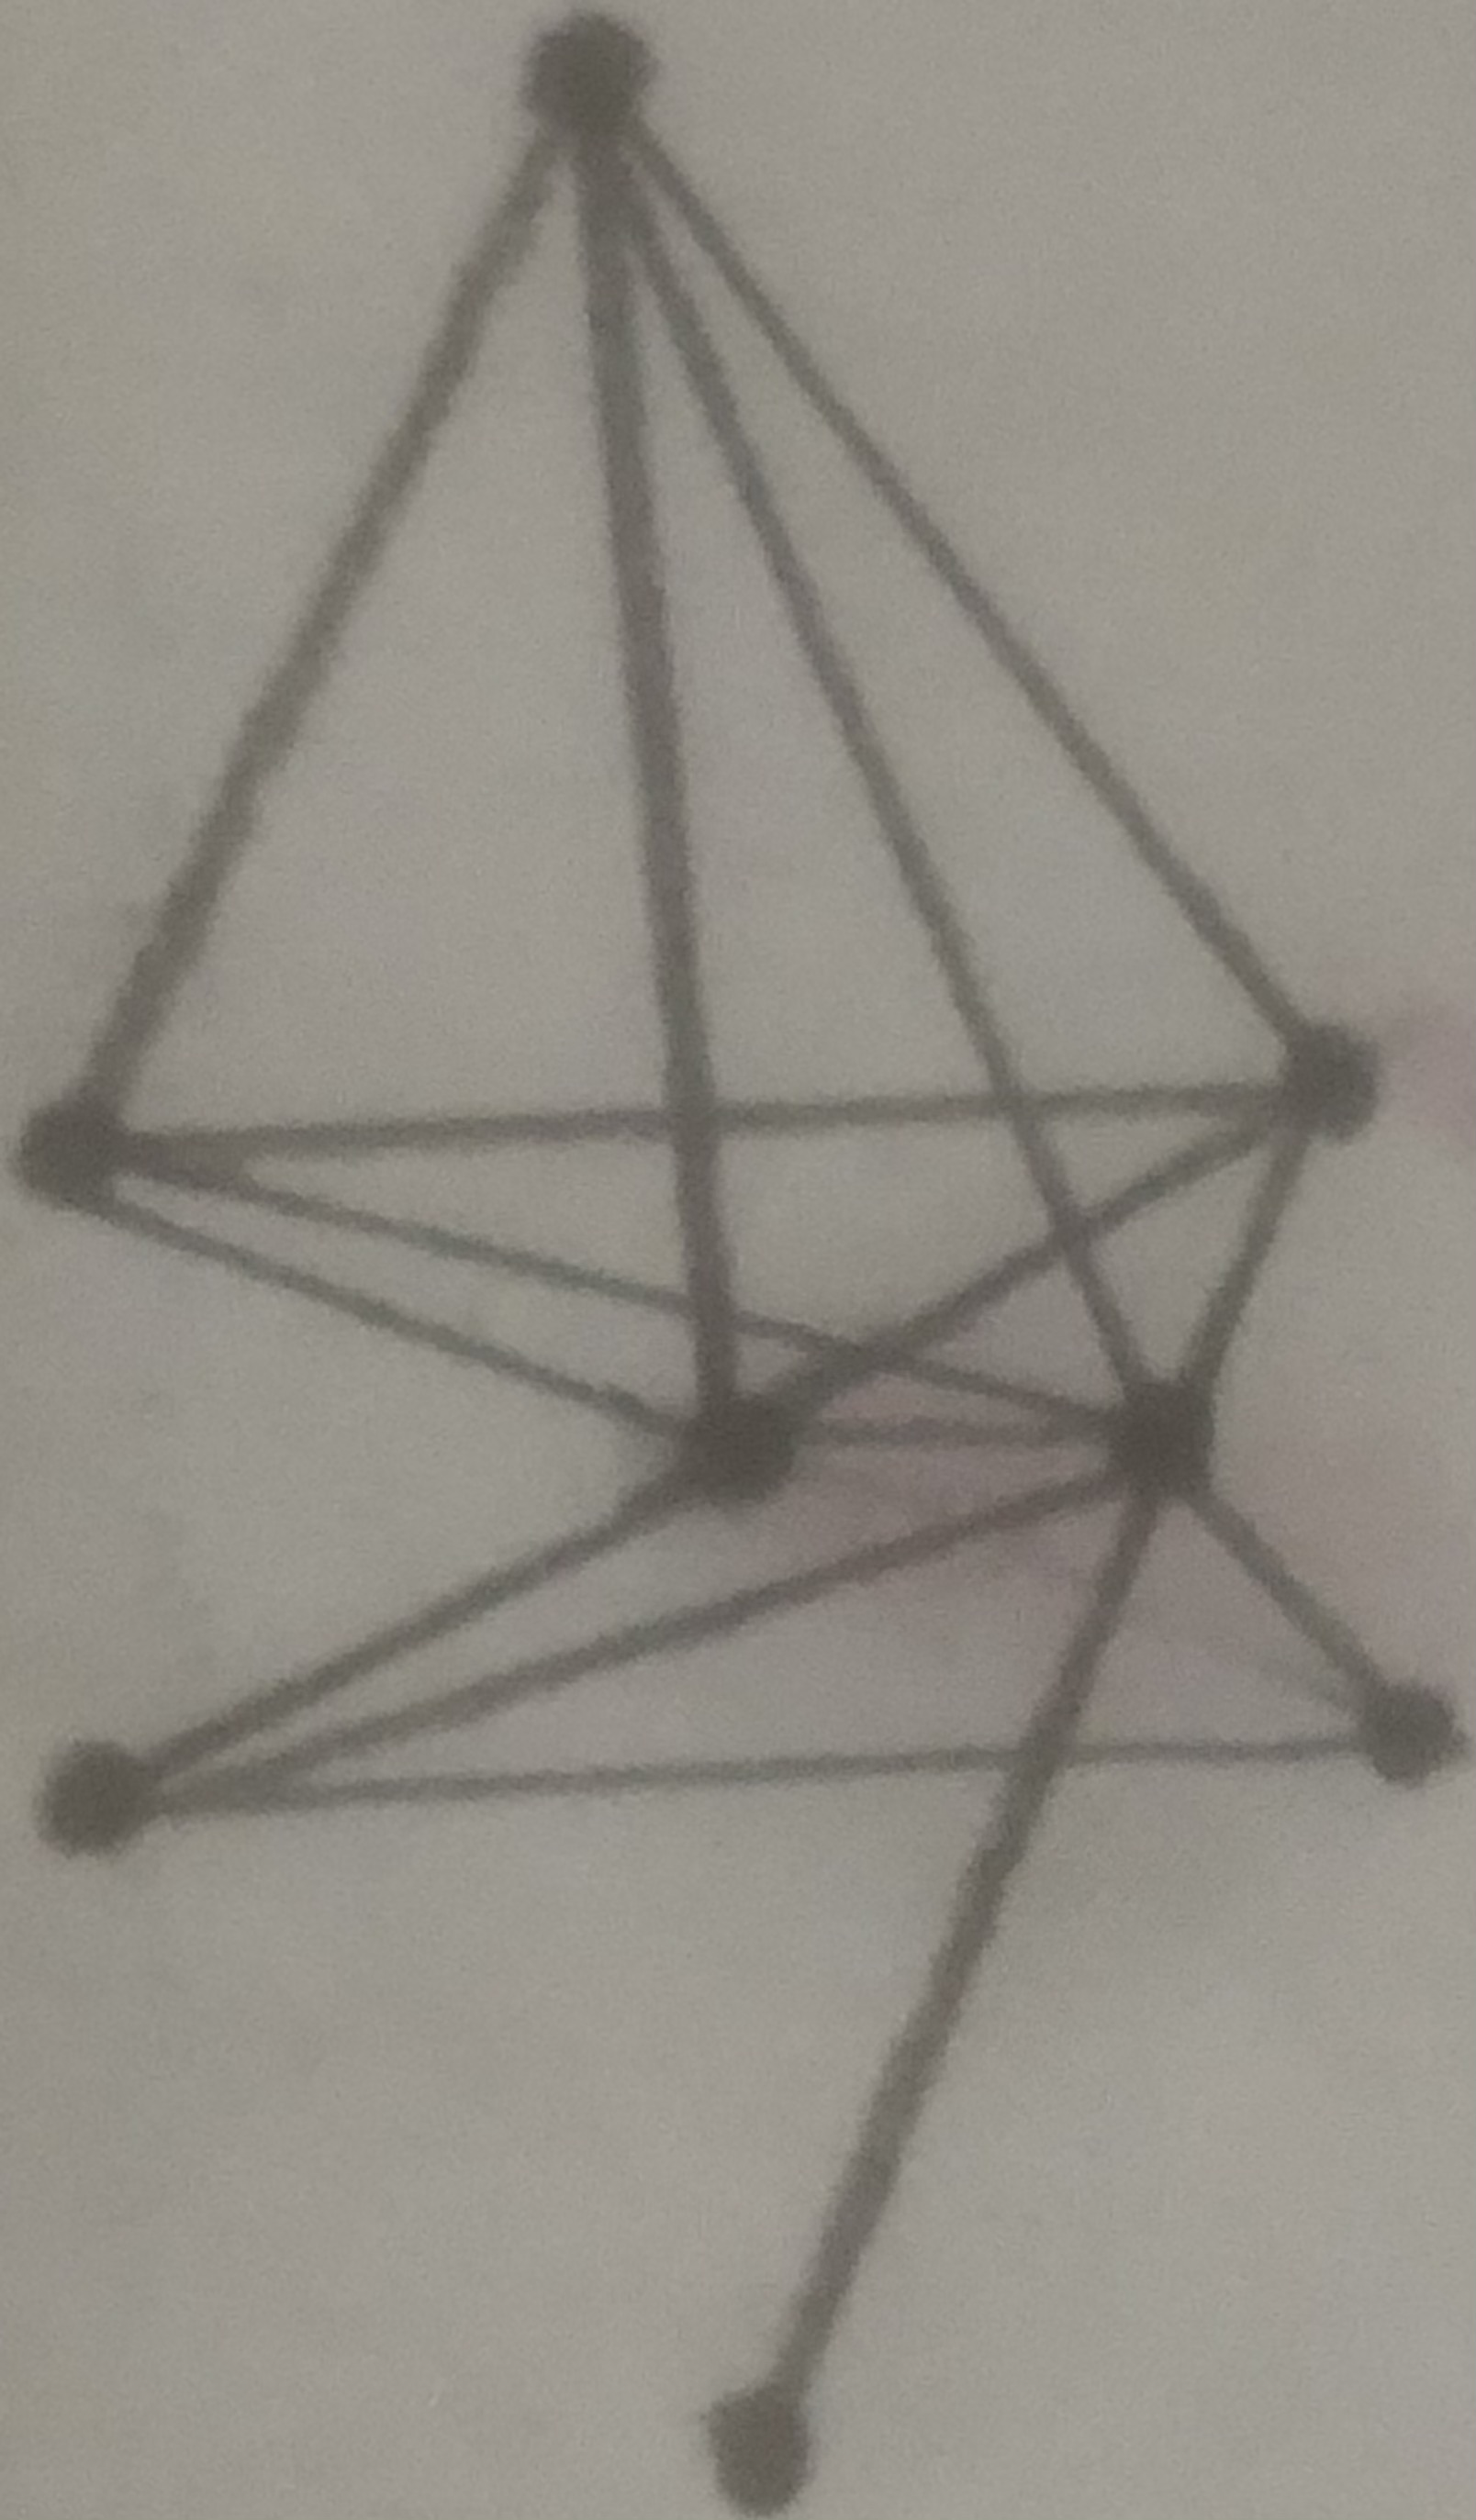
\includegraphics[width=3cm]{IMG-0785.JPG}
\end{center}

\medskip{\bf (e)}
\begin{align*}
    s_5    &= (7,6,5,4,4,3,2,1) \\
    s_5'   &=   (5,4,3,3,2,1,0) \\
    s_5''  &=     (3,2,2,1,0,0) \\
    s_5''' &=       (1,1,0,0,0)
\end{align*} Since $s_5'''$ is the degree sequence of $K_2 \cup N_3$, $s_5$ is graphical.

Shown left to right are graphs corresponding to $s_5'''$, $s_5''$, $s_5'$, and $s_5$:
\begin{center}
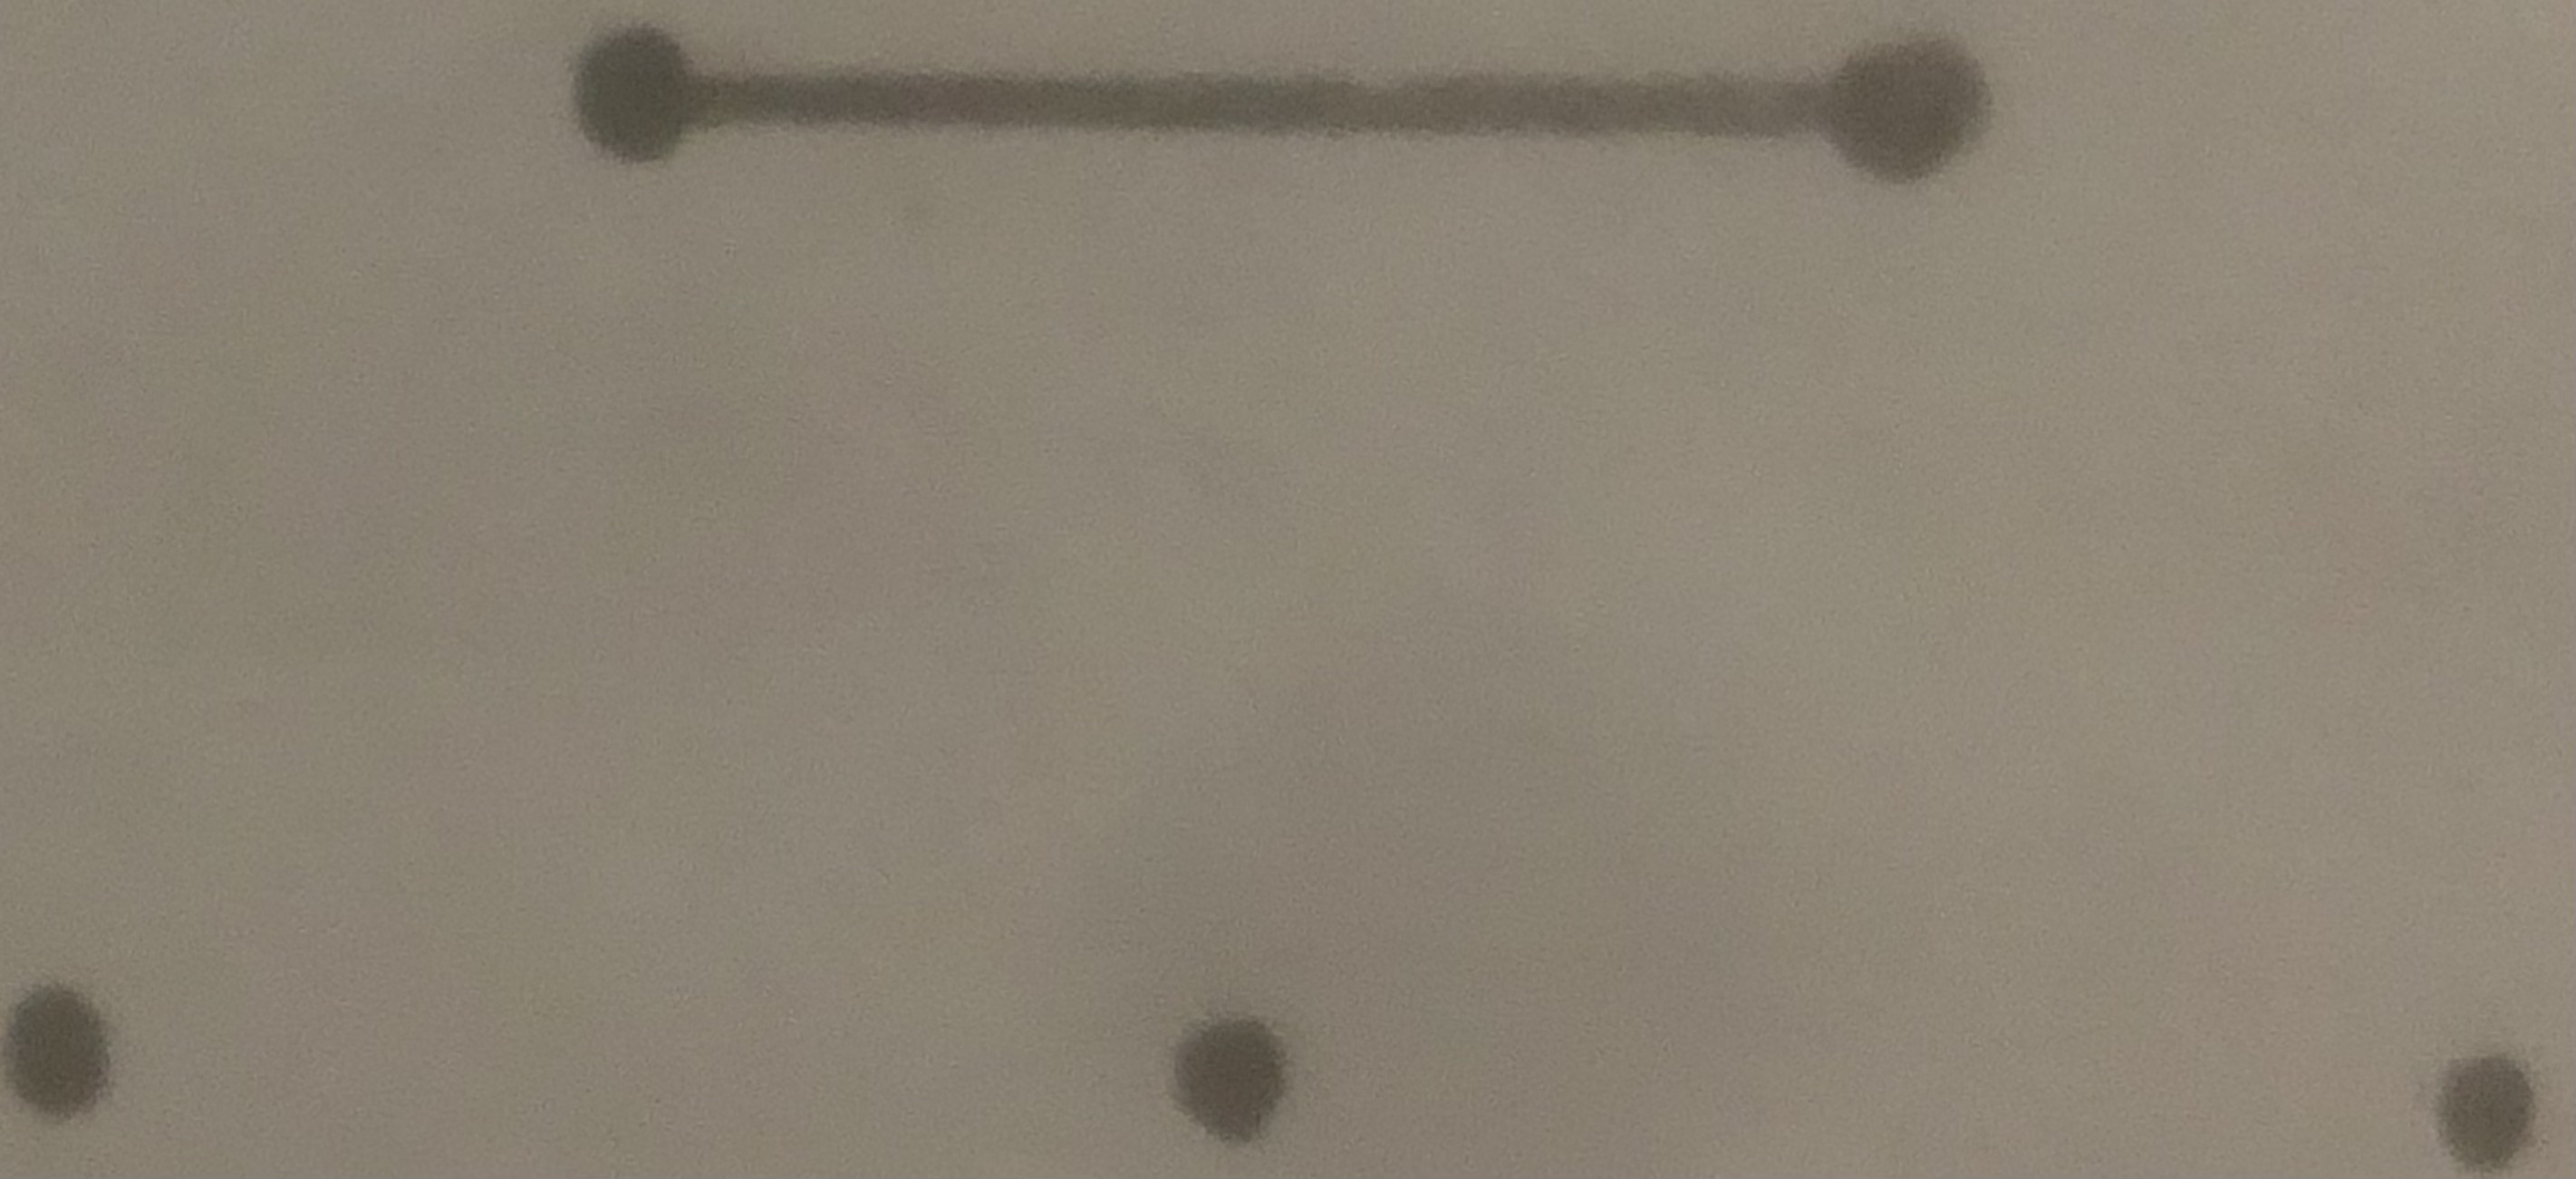
\includegraphics[width=3cm]{IMG-0786.JPG}
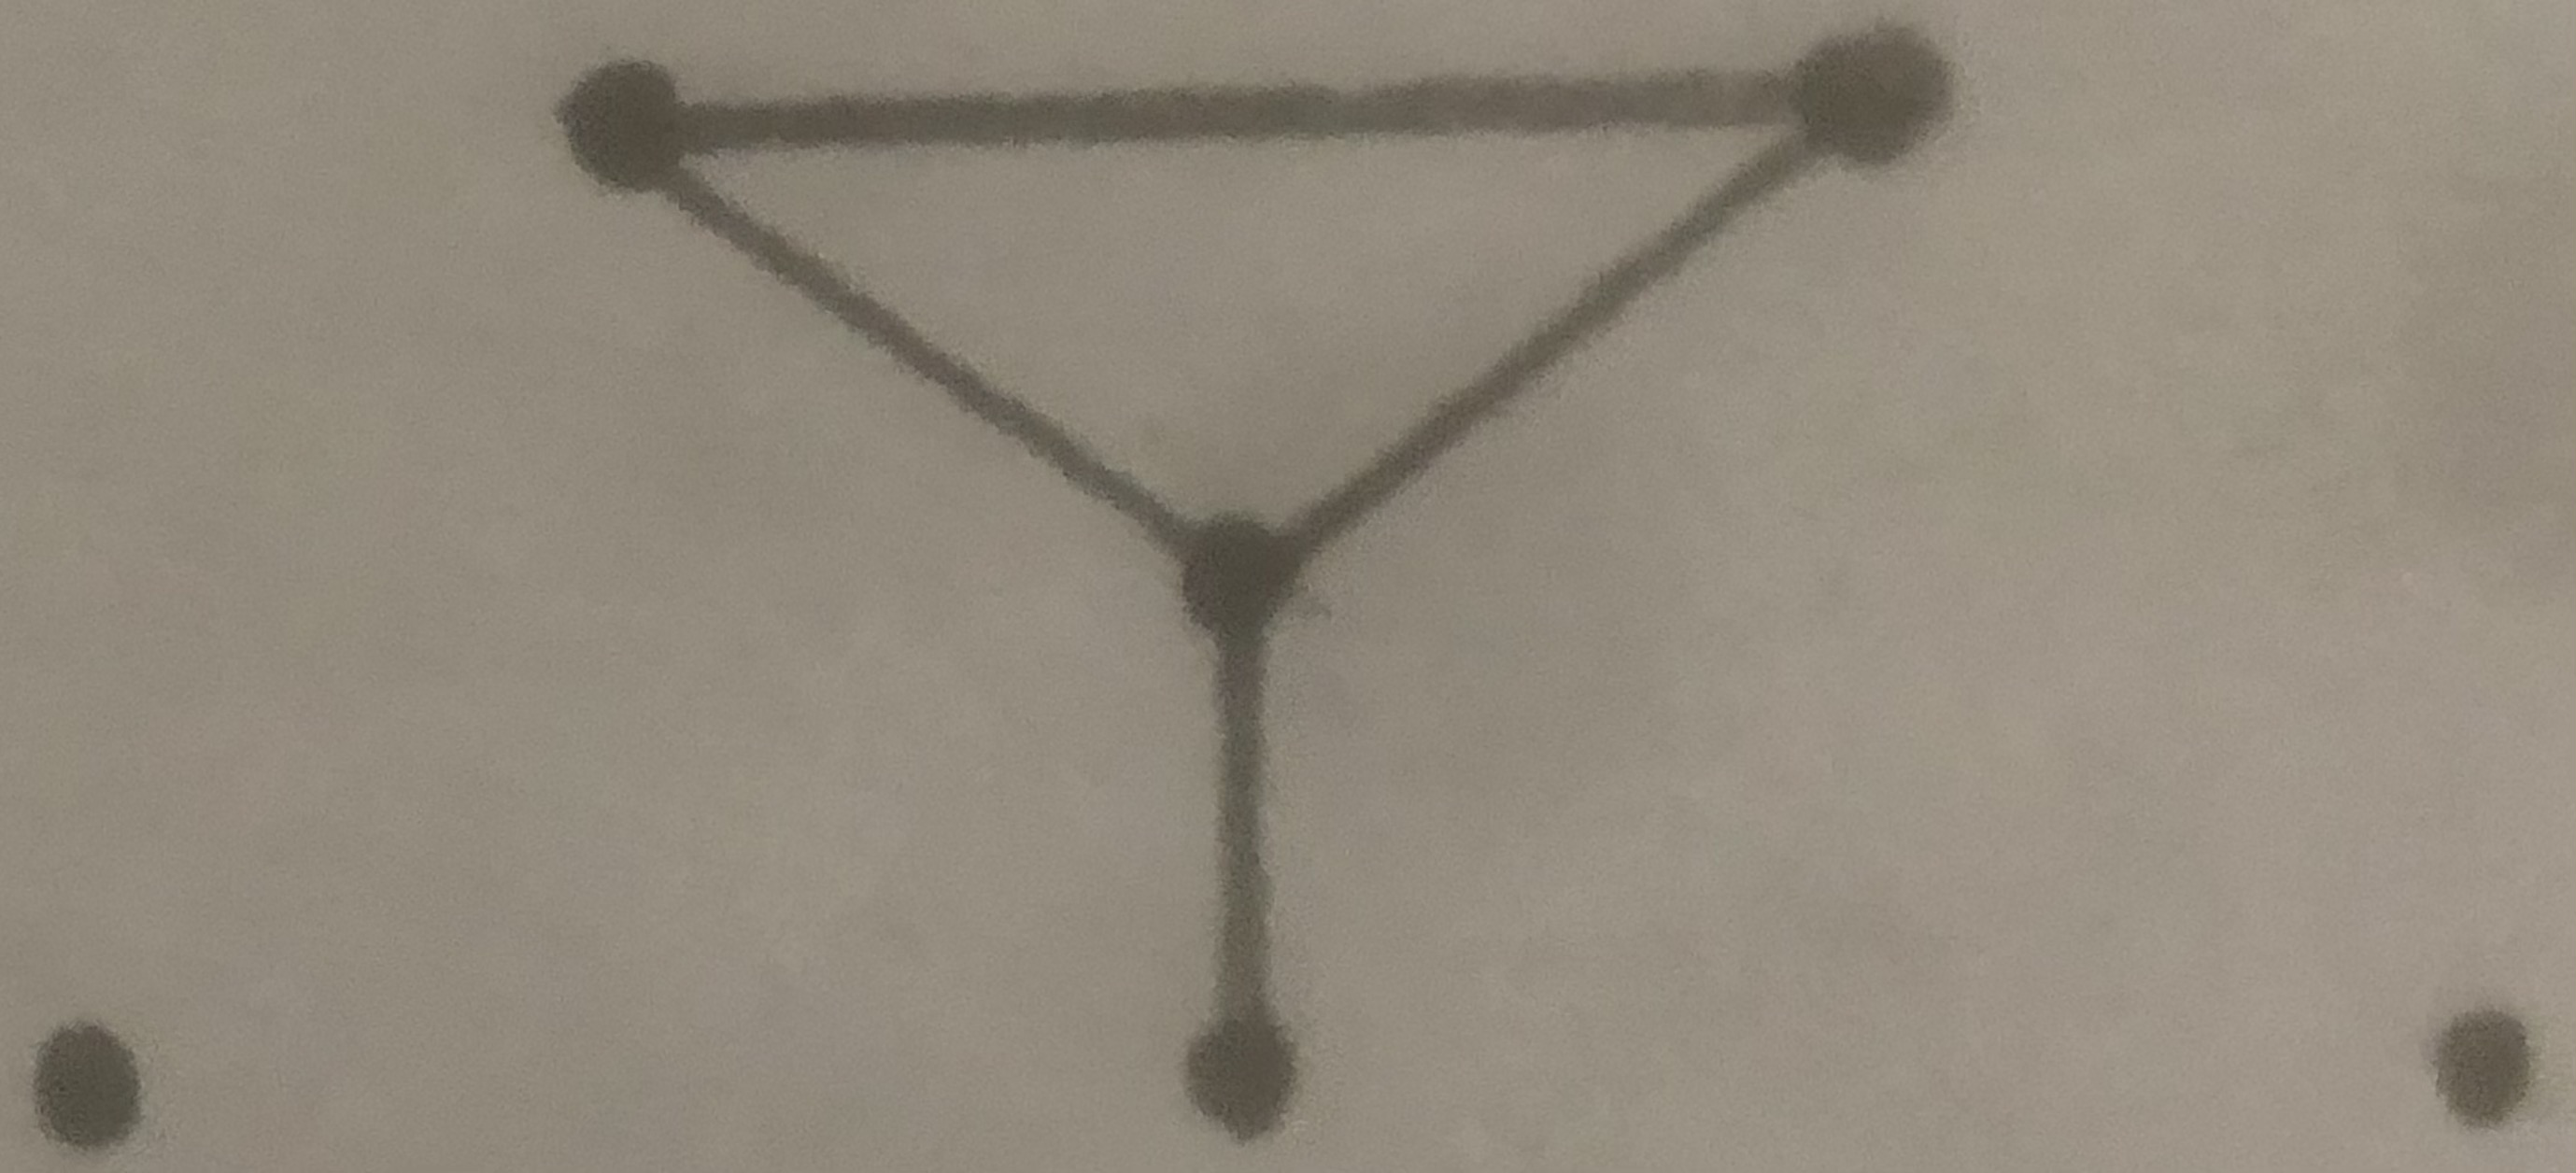
\includegraphics[width=3cm]{IMG-0787.JPG}
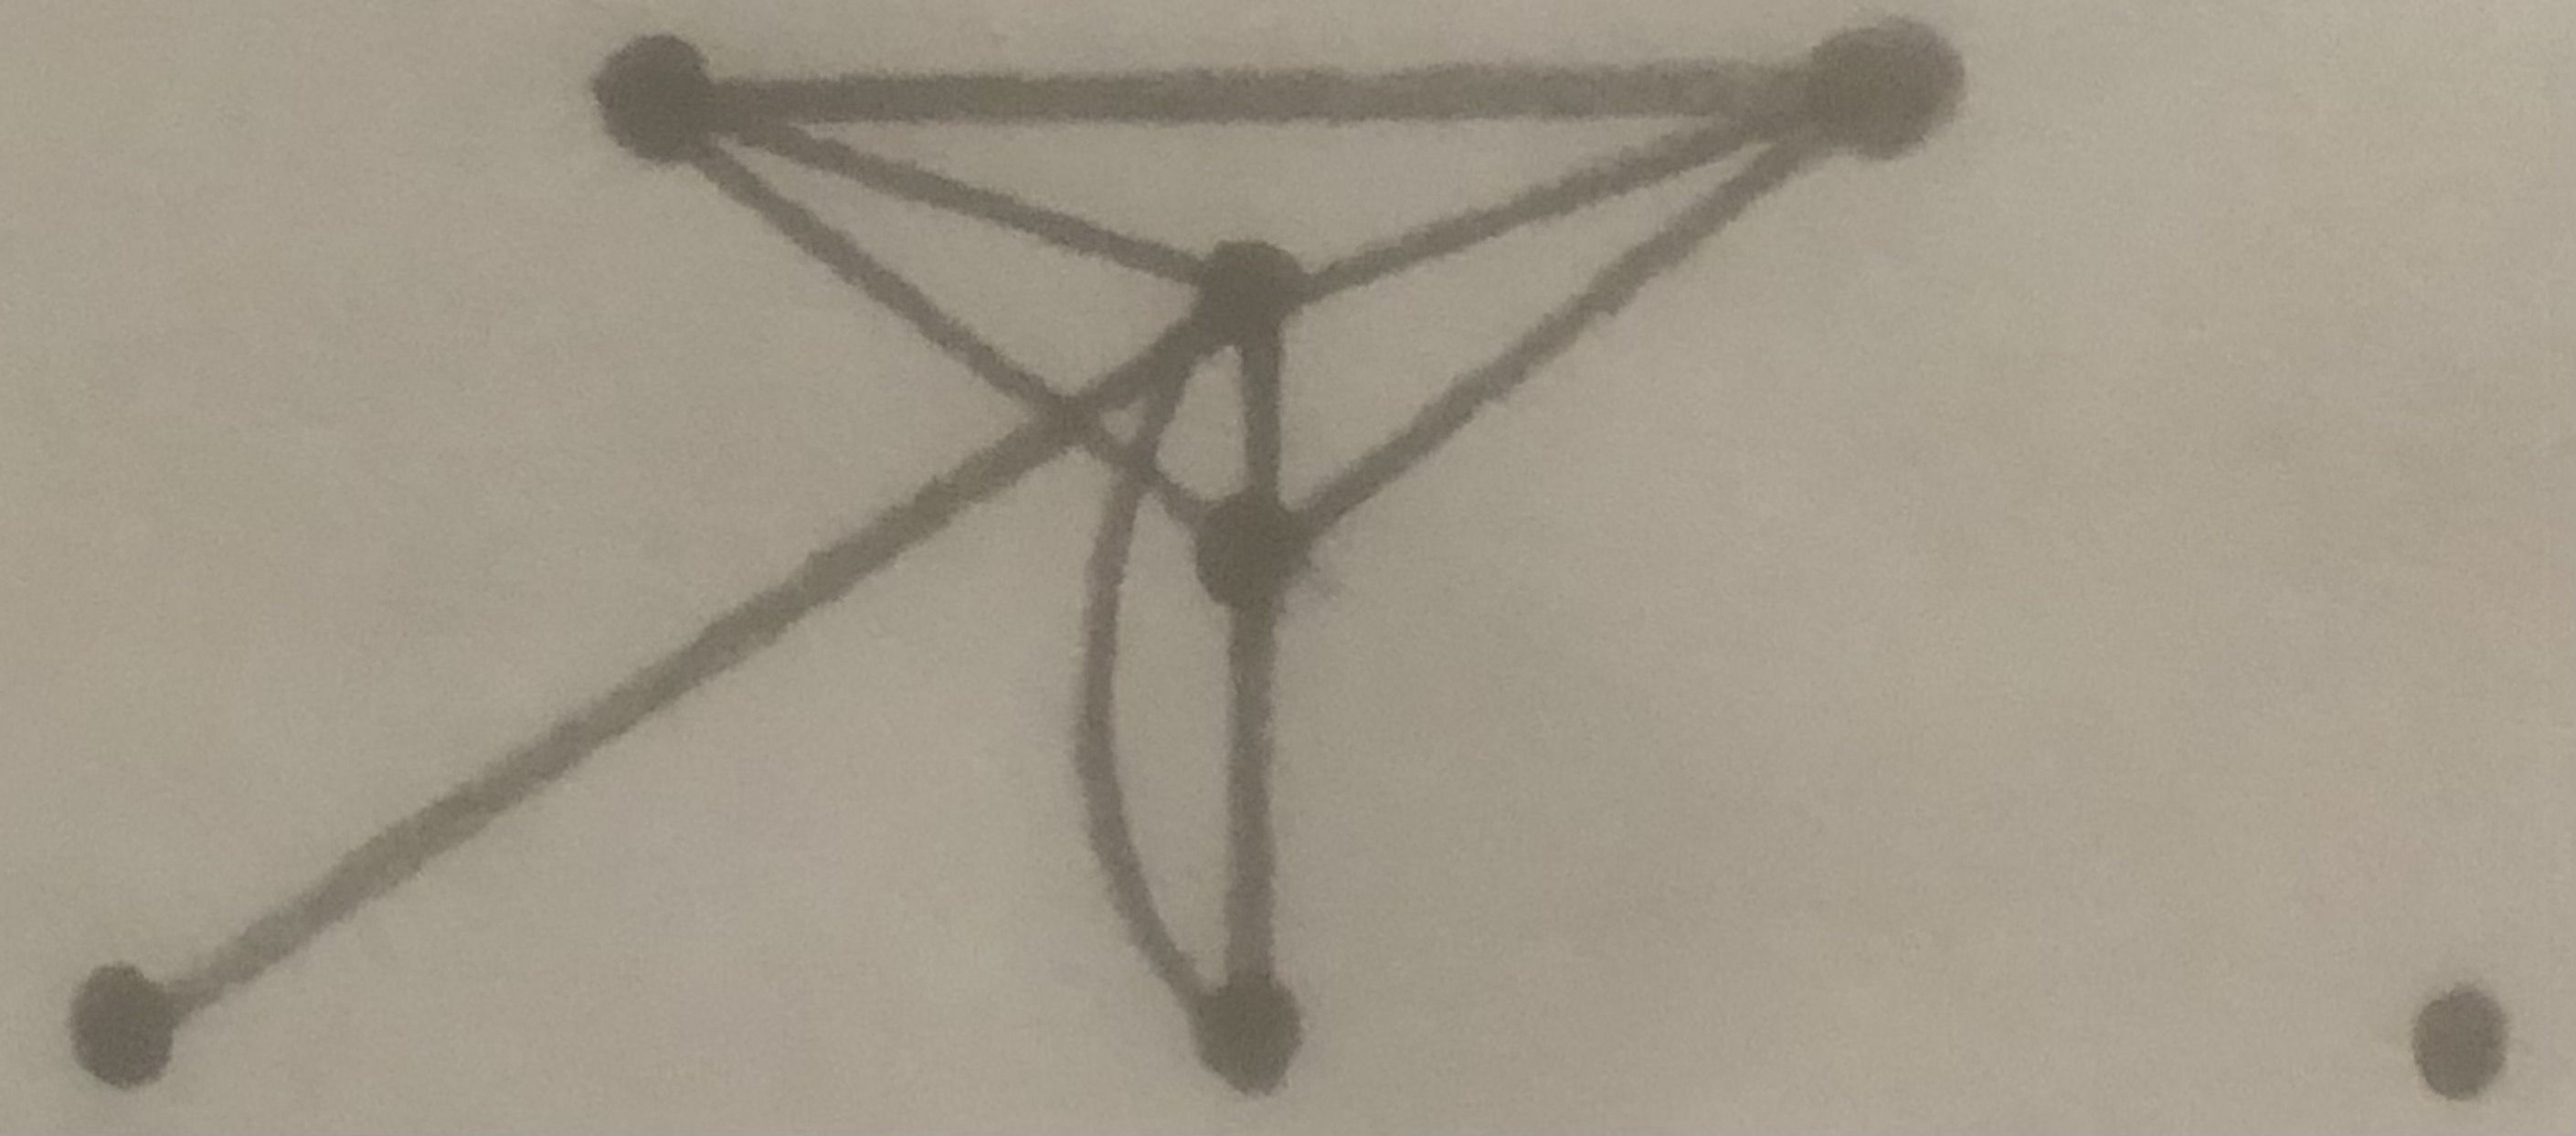
\includegraphics[width=3cm]{IMG-0788.JPG}
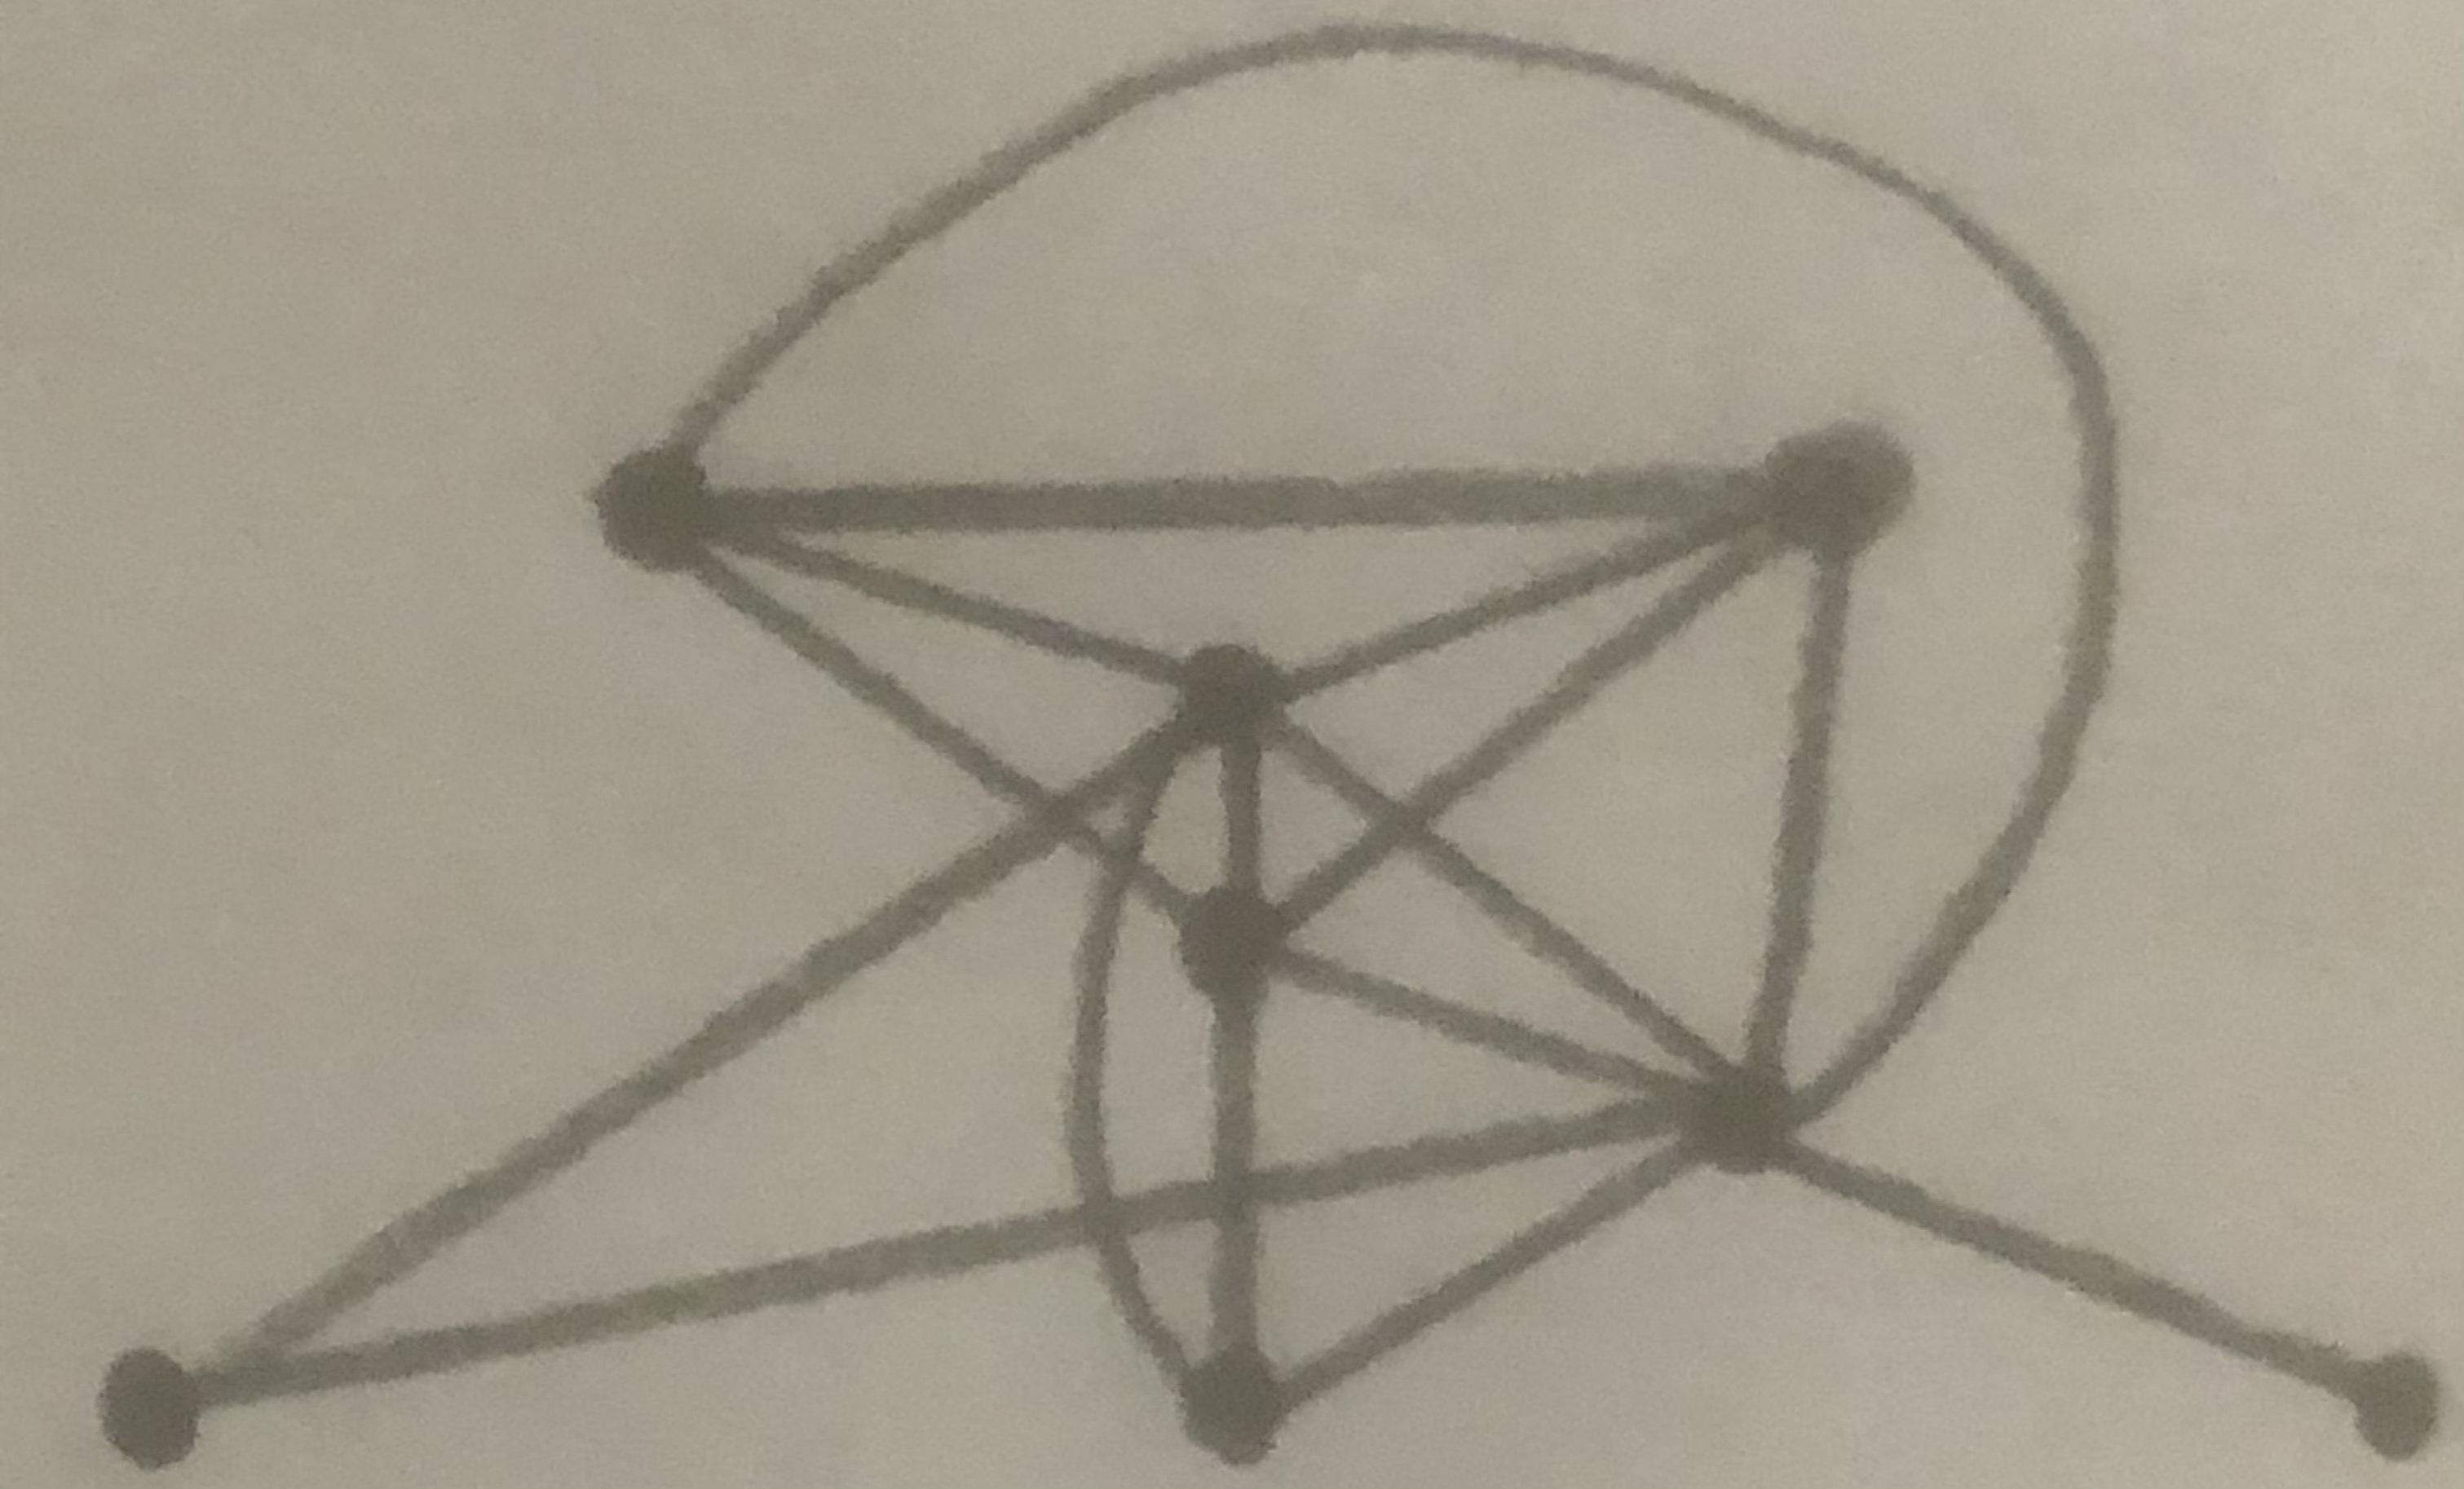
\includegraphics[width=3cm]{IMG-0789.JPG}
\end{center}

\newpage\noindent{\bf 2.36} Proposition: The smallest positive integer $k$ such that the sequence obtained by listing each element of $\{2,6,7\}$ a total of $k$ times is a degree sequence of some graph is 4.
\begin{proof}
    Let $S = \{2,6,7\}$.
    Let $k$ be the smallest positive integer such that the sequence obtained by listing each element of $S$ a total of $k$ times is a degree sequence of some graph.
    Since $7 \in S$, any graph with a degree sequence of the desired form must have at least 8 vertices.
    Thus, $k \cdot |S| \geq 8$, so $k \geq 3$.
    Observe that $k \neq 3$, since the sequence generated by listing each element of $S$ a total of three times has a total of 3 odd entries, and is thus not a graphical sequence by Corollary 2.3.

    Let $s$ be the sequence obtained by listing each element of $S$ a total of four times.
    Then, $s = (7,7,7,7,6,6,6,6,2,2,2,2)$.
    Thus, by Theorem 2.10, $s$ is graphical if and only if the following sequences are graphical:
    \begin{align*}
        s_1 &= (6,6,6,5,5,5,5,2,2,2,2) \\
        s_2 &=   (5,5,4,4,4,4,2,2,2,2) \\
        s_3 &=     (4,3,3,3,3,2,2,2,2) \\
        s_4 &=       (2,2,2,2,2,2,2,2)
    \end{align*}
    Since $s_4$ is the degree sequence of $C_8$, $s_4$ is graphical.
    Thus, $s$ is graphical.
    Therefore, the smallest positive integer $k$ such that the sequence obtained by listing each element of $\{2,6,7\}$ a total of $k$ times is a degree sequence of some graph is 4.
\end{proof}

\newpage\noindent{\bf 2.37}

Since $v_1, v_2, v_3$ are in symmetric positions in $G_1$, and so are $v_4, v_5$, we need only enumerate the following length two walks to compute $A^2$:
\begin{align*}
    v_1 \to v_1 &: \{(v_1, v_5, v_1), (v_1, v_4, v_1)\} \\
    v_1 \to v_2 &: \{(v_1, v_5, v_2), (v_1, v_4, v_2)\} \\
    v_1 \to v_4 &: \{(v_1, v_5, v_4)\} \\
    v_4 \to v_4 &: \{(v_4, v_1, v_4), (v_4, v_2, v_4), (v_4, v_3, v_4), (v_4, v_5, v_4)\} \\
    v_4 \to v_5 &: \{(v_4, v_3, v_5), (v_4, v_2, v_5), (v_4, v_1, v_5)\} \\
\end{align*}
Thus, $$A^2 = \begin{bmatrix}
                2 & 2 & 2 & 1 & 1 \\
                2 & 2 & 2 & 1 & 1 \\
                2 & 2 & 2 & 1 & 1 \\
                1 & 1 & 1 & 4 & 3 \\
                1 & 1 & 1 & 3 & 4
              \end{bmatrix}$$

Since $v_1, v_2, v_3$ are in symmetric positions in $G_1$, and so are $v_4, v_5$, we need only enumerate the following length three walks to compute $A^3$:
\begin{align*}
    v_1 \to v_1 &: \{(v_1, v_4, v_5, v_1), (v_1, v_5, v_4, v_1)\} \\
    v_1 \to v_2 &: \{(v_1, v_4, v_5, v_2), (v_1, v_5, v_4, v_2)\} \\
    v_1 \to v_4 &: \{(v_1, v_4, v_1, v_4), (v_1, v_4, v_3, v_4), (v_1, v_4, v_2, v_4), (v_1, v_4, v_5, v_4), (v_1, v_5, v_1, v_4), (v_1, v_5, v_3, v_4), (v_1, v_5, v_2, v_4)\} \\
    v_4 \to v_4 &: \{(v_4, v_1, v_5, v_4), (v_4, v_2, v_5, v_4), (v_4, v_3, v_5, v_4), (v_4, v_1, v_5, v_4), (v_4, v_2, v_5, v_4), (v_4, v_3, v_5, v_4)\}
\end{align*}
Thus, $$A^3 = \begin{bmatrix}
                2 & 2 & 2 & 7 & 7 \\
                2 & 2 & 2 & 7 & 7 \\
                2 & 2 & 2 & 7 & 7 \\
                7 & 7 & 7 & 6 & 7 \\
                7 & 7 & 7 & 7 & 6
              \end{bmatrix}$$

\newpage\noindent{\bf 2.39}

Since $v_1, v_2$ are symmetric to $v_4, v_3$ in $G_3$, we need only enumerate the following length four walks to compute $A^4$:
\begin{align*}
    v_1 \to v_1 &: \{(v_1, v_2, v_1, v_2, v_1), (v_1, v_2, v_3, v_2, v_1)\} \\
    v_1 \to v_2 &: \{\} \\
    v_1 \to v_3 &: \{(v_1, v_2, v_3, v_2, v_3), (v_1, v_2, v_1, v_2, v_3), (v_1, v_2, v_3, v_4, v_3)\} \\
    v_1 \to v_4 &: \{\} \\
    v_2 \to v_2 &: \{(v_2, v_3, v_4, v_3, v_2), (v_2, v_1, v_2, v_3, v_2), (v_2, v_1, v_2, v_1, v_2), (v_2, v_3, v_2, v_1, v_2), (v_2, v_3, v_2, v_3, v_2)\} \\
    v_2 \to v_3 &: \{\} \\
    v_2 \to v_4 &: \{(v_2, v_1, v_2, v_3, v_4), (v_2, v_3, v_2, v_3, v_4), (v_2, v_3, v_4, v_3, v_4)\}
\end{align*}
Thus, $$A^4 = \begin{bmatrix}
                2 & 0 & 3 & 0 \\
                0 & 5 & 0 & 3 \\
                3 & 0 & 5 & 0 \\
                0 & 3 & 0 & 2 \\
              \end{bmatrix}$$

\newpage\noindent{\bf 2.40} \\
$A = ~~v_1\hspace*{5mm}\dots\hspace*{1mm} v_rv_{r+1}\hspace*{2mm}\dots\hspace*{1mm}v_{2r}\\
\hspace*{10mm}\begin{bmatrix}
0&\dots&0&1&\dots&1\\
\vdots&\vdots&\vdots&\vdots&\vdots&\vdots\\
0&\dots&0&1&\dots&1\\
1&\dots&1&0&\dots&0\\
\vdots&\vdots&\vdots&\vdots&\vdots&\vdots\\
1&\dots&1&0&\dots&0\\
\end{bmatrix}$,\\
$A^2 = \,v_1\hspace*{5mm}\dots\hspace*{1mm} v_rv_{r+1}\hspace*{2mm}\dots\hspace*{1mm}v_{2r}\\
\hspace*{10mm}\begin{bmatrix}
r&\dots&r&0&\dots&0\\
\vdots&\vdots&\vdots&\vdots&\vdots&\vdots\\
r&\dots&r&0&\dots&0\\
0&\dots&0&r&\dots&r\\
\vdots&\vdots&\vdots&\vdots&\vdots&\vdots\\
0&\dots&0&r&\dots&r\\
\end{bmatrix}$,\\
$A^3 = \,\,\,v_1\hspace*{5mm}\dots\hspace*{1mm} v_rv_{r+1}\hspace*{2mm}\dots\hspace*{1mm}v_{2r}\\
\hspace*{10mm}\begin{bmatrix}
0&\dots&0&r^2&\dots&r^2\\
\vdots&\vdots&\vdots&\vdots&\vdots&\vdots\\
0&\dots&0&r^2&\dots&r^2\\
r^2&\dots&r^2&0&\dots&0\\
\vdots&\vdots&\vdots&\vdots&\vdots&\vdots\\
r^2&\dots&r^2&0&\dots&0\\
\end{bmatrix}$,\\
$A^4 = \,\,\,v_1\hspace*{5mm}\dots\hspace*{1mm} v_rv_{r+1}\hspace*{2mm}\dots\hspace*{1mm}v_{2r}\\
\hspace*{10mm}\begin{bmatrix}
r^3&\dots&r^3&0&\dots&0\\
\vdots&\vdots&\vdots&\vdots&\vdots&\vdots\\
r^3&\dots&r^3&0&\dots&0\\
0&\dots&0&r^3&\dots&r^3\\
\vdots&\vdots&\vdots&\vdots&\vdots&\vdots\\
0&\dots&0&r^3&\dots&r^3\\
\end{bmatrix}$\\

A bipartite graph has no odd-length walks between two vertices in the same partite set. Thus, for odd $n$, all entries that correspond to walks between vertices in the same partite set are zeros in $A^n$.
Similarly, for even $n$, all entries that correspond to walks between vertices in different partite sets are zeros in $A^n$.
All other entries in $A^n$ are $r^{n-1}$.
This is because each vertex in $G$ is of degree $r$, so there are $r$ choices for each of edge in any given path.
\newpage\noindent{\bf 2.41}

\medskip{\bf (a)}
$$BB^T = \begin{bmatrix}
3&1&1&1&0\\
1&2&0&1&0\\
1&0&2&1&0\\
1&1&1&4&1\\
0&0&0&1&1
\end{bmatrix}$$

\medskip{\bf (b)} The $ij^{\text{th}}$ entry of $BB^T$ is the number of edges $e$ in $G$ satisfying $\{i,j\} \subseteq e$.

    The $ij^{\text{th}}$ entry of $BB^T$ is equal to the dot product of the $i^{\text{th}}$ row of $B$ and the $j^{\text{th}}$ column of $B^T$.
    Thus, $ij^{\text{th}}$ entry of $BB^T$ is equal to the dot product of the $i^{\text{th}}$ row of $B$ and the $j^{\text{th}}$ row of $B$.
    Since $B$'s entries are all 0 or 1, the $ij^{\text{th}}$ entry of $B$ is equal to the number of edges in $G$ containing both $i$ and $j$.
    Thus, if $i \neq j$, then $ij^{\text{th}}$ entry of $B$ is 1 if and only if $ij \in E(G)$, and if $i=j$, then $ij^{\text{th}}$ entry of $B$ is the degree of $i$ in $G$.

\end{document}